\documentclass[11pt,twoside,a4paper]{article}
\usepackage[hmargin=2cm, vmargin=2cm]{geometry}
\usepackage{microtype}
\usepackage{graphicx}
\usepackage[english]{babel}
\usepackage{setspace}
\usepackage{xcolor}
\usepackage{multicol}
\usepackage{float}
\usepackage{amsmath}
\usepackage{amsthm}
\usepackage{amssymb}
\usepackage[hidelinks=true]{hyperref}
\usepackage{overpic}
\usepackage[font=small,skip=2pt]{caption}
\usepackage[
backend=biber,
style=authoryear-comp,
]{biblatex}

\newcommand{\independent}{\perp\!\!\!\!\perp} 

\addbibresource{RMbibliography.bib}
\onehalfspacing
\parindent=0pt
\usepackage{pagecolor}
\pagecolor{white}
\begin{document}

\begin{titlepage}
    \centering
    {\LARGE\bfseries Dimension Reduction in Regression: \\ Comparative Analysis of Principal Component Regression and Partial Least Squares\par}
    \vspace{1.5cm}
    
    {\Large Khabibullo Ibadullaev, Bekhzod Abulov\par}
    \vspace{0.5cm}
    
    {\large \today\par}
    \vspace{3cm}
    
    {\large University of Bonn\par}
    {\large Research Module in Econometrics and Statistics\par}
    {\large Supervised by: Prof. Dr. Joachim Freyberger\par}
    
    \vspace{0.5cm}
    
    {\large Winter Semester 2024/2025\par}
\end{titlepage}

\newpage

\thispagestyle{empty}
\tableofcontents

\newpage

\setlength{\abovedisplayskip}{0.35cm}
\setlength{\belowdisplayskip}{0.35cm}

\setlength{\abovedisplayshortskip}{0.2cm}
\setlength{\belowdisplayshortskip}{0.35cm}
\setlength{\parskip}{0.5em}
\pagenumbering{arabic}

\section{Introduction}

Regression models are a fundamental tool in statistical modeling, enabling the prediction of a dependent variable based on a set of independent variables. However, in modern applications, datasets often exhibit high-dimensionality, where the number of predictors (\( p \)) is significantly larger than the number of observations (\( n \)). This scenario, commonly referred to as the curse of dimensionality, poses significant challenges to traditional regression methods, particularly Ordinary Least Squares (OLS) regression.

One of the primary concerns in high-dimensional regression is multicollinearity—a situation where predictor variables are highly correlated. Multicollinearity leads to inflated standard errors, unstable coefficient estimates, and difficulties in interpreting model parameters. Additionally, high-dimensional models tend to overfit the training data, resulting in poor generalization to unseen observations. Computational complexity further exacerbates these challenges, making it difficult to estimate model parameters efficiently.
To address these issues, researchers have developed dimension reduction techniques that aim to transform high-dimensional predictor spaces into lower-dimensional representations while preserving essential information. Two widely used techniques in this context are Principal Component Regression (PCR) and Partial Least Squares (PLS). These methods construct new predictor variables, referred to as components, that capture the most relevant variation in the dataset.
The use of PCR and PLS is prevalent in various disciplines, including chemometrics, finance, genomics, and environmental science, where datasets often contain a large number of correlated predictors. While both methods offer solutions to the high-dimensional regression problem, they differ in their approach, underlying assumptions, and effectiveness in different scenarios.

This paper provides a comprehensive analysis of  Principal Component Regression (PCR) and Partial Least Squares (PLS), focusing on their theoretical foundations, practical implementations, and empirical performance evaluation across various regression settings. Specifically, in Section 2 we investigate the mathematical principles underlying these methods, highlighting their similarities and differences in handling multicollinearity and dimensionality reduction. A key focus in Section 3 is on understanding the bias-variance trade-off by performing a detailed Mean Squared Error (MSE) decomposition of regression coefficients, as well as evaluating predictive performance through Cross-Validation (CV) MSE. The study systematically compares these methods in different scenarios. To further assess model stability and generalization ability, a Monte Carlo simulation is conducted using synthetic datasets, allowing for an in-depth examination of performance under varying levels of correlation. Additionally, in Section 4 both PCR and PLS are applied to real-world regression problems, including Near-Infrared (NIR) Spectroscopy for Moisture Prediction, to evaluate their practical utility and interpretability. Finally, in Section 5 we discuss the strengths and weaknesses of each method, providing guidance on when to prefer PCR over PLS (or vice versa) and exploring potential hybrid approaches that integrate the advantages of both techniques.
\newpage

\section{Theory}

Traditional regression methods, such as OLS, assume that the predictor matrix \( X \) has full rank, ensuring a unique solution for the estimated coefficients. However, in many practical applications, datasets exhibit high collinearity among predictors or even contain more predictors than observations (\( p \gg n \)), making \( X^T X \) nearly singular or non-invertible. This leads to large variances in coefficient estimates, making the regression model highly unstable. The instability of OLS is evident in the variance expression:
\begin{equation} 
\text{Var}(\hat{\beta}_{\text{OLS}}) = \sigma^2 (X^T X)^{-1}
\end{equation}
Applying the eigen-decomposition:
\begin{equation}
X^T X = Q \Lambda Q^T
\end{equation}
we obtain:
\begin{equation}
\text{Var}(\hat{\beta}_{\text{OLS}}) = \sigma^2 Q \Lambda^{-1} Q^T
\end{equation}
where \( \Lambda \) contains the eigenvalues of \( X^T X \), we observe that when multicollinearity is present, some eigenvalues approach zero, making \( \Lambda^{-1} \) contain large values, which significantly inflates the variance of \( \hat{\beta}_{\text{OLS}} \).

PCR and PLS overcome this issue by constructing a set of orthogonal predictors, thereby improving numerical stability and reducing overfitting. While,  PCR mitigates this issue by removing components corresponding to small eigenvalues, ensuring that the variance of the estimated coefficients remains controlled, PLS focuses on components that maximize the covariance with \( Y \), eliminating high-variance directions that contribute to unstable coefficient estimates, ensuring a more robust regression model.


\subsection{Principal Component Regression (PCR)}

Principal Component Regression (PCR) is a widely used statistical technique that integrates Principal Component Analysis (PCA) with Ordinary Least Squares (OLS) regression to address issues of high-dimensionality and multicollinearity in regression problems. The fundamental idea behind PCR is to transform the original predictor variables, which may be highly correlated, into a new set of uncorrelated variables called principal components (Figure 1). Regression is then performed using a selected subset of these principal components, effectively reducing the dimensionality of the predictor space while mitigating instability in coefficient estimates.

PCR is an effective tool for dealing with multicollinearity, it is important to note that it is an unsupervised method, meaning that the principal components are chosen solely based on variance in the predictor space, without considering the response variable \( Y \). This characteristic distinguishes it from methods like Partial Least Squares (PLS), which optimize component selection based on predictive relevance to \( Y \).

\paragraph{Mathematical Formulation} \ \

The key steps of PCR are as follows:

\begin{enumerate}
    \item Perform \textbf{Principal Component Analysis (PCA)} on \( X \), which involves computing the \textbf{Singular Value Decomposition (SVD)}:
   \begin{equation}
    X = U \Sigma V^T
    \end{equation}
    where:
    \begin{itemize}
        \item \( U \) is an \( n \times n \) orthogonal matrix (left singular vectors),
        \item \( \Sigma \) is an \( n \times p \) diagonal matrix with singular values,
        \item \( V \) is a \( p \times p \) orthogonal matrix (right singular vectors), whose columns are the principal component directions.
    \end{itemize}
    
    \item Transform the original predictors into principal components:
    \begin{equation}
    Z = X V
    \end{equation}
 
    \item Perform OLS regression on the transformed dataset:
    \begin{equation}
    Y = Z \gamma + \epsilon
    \end{equation}
    where \( \gamma \) is the transformed coefficient vector in the principal component space.
  \end{enumerate}
  
 \paragraph{Unsupervised Nature of PCR} \ \

PCR is fundamentally an \textbf{unsupervised} technique because it selects principal components based on variance in \( X \) without considering \( Y \). This is evident from the PCA decomposition:
\begin{equation}
X^T X = V \Lambda V^T
\end{equation}
Since \( V \) is computed purely from \( X \), it does not incorporate \( Y \). As a result, PCR may discard components that contain important predictive information for \( Y \), making it less efficient for regression tasks compared to supervised alternatives like PLS.

\begin{figure}[H]
    \centering
    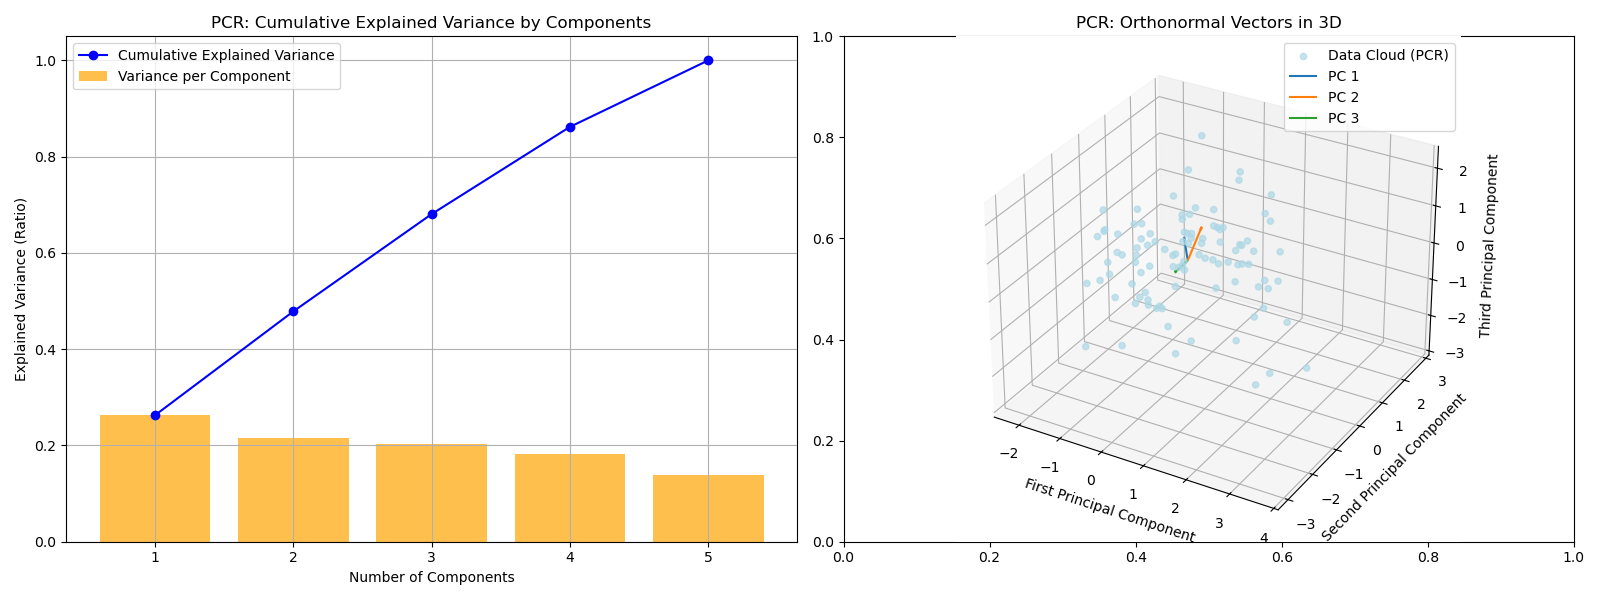
\includegraphics[width=0.9\textwidth]{PCR_Selected_Analysis.png}
    \caption{Principal Component Regression (PCR) Analysis Results}
    \label{fig:PCR_analysis}
\end{figure}

\paragraph{Variance Reduction and Bias in PCR}  \ \

A key feature of PCR is its ability to reduce variance in estimated coefficients by using only first \( k \) principal components and eliminating components associated with small eigenvalues:
   \begin{equation}
    Z_k = X V_k
    \end{equation}
    \begin{equation}
\hat{\gamma_k} = (Z_k^T Z_k)^{-1} Z_k^T Y
\end{equation}
\begin{equation}
\hat{\gamma_k}  = \Lambda_k^{-1} V_k^T X^T Y
\end{equation}
    where \( \Lambda_k \) contains only the top \( k \) eigenvalues of \( X^T X \), while \( V_k \) consists of the first \( k \) principal components that capture the most variance in \( X \). The selection of \( k \) is often done using cross-validation or based on the cumulative explained variance criterion (Figure 1).

Transforming back to the original space:
\begin{equation}
\hat{\beta}_{\text{PCR}} = V_k \hat{\gamma_k} = V_k \Lambda_k^{-1} V_k^T X^T Y
\end{equation}
Recall that OLS can be written in terms of PCA decomposition (7). If all principal components are used (\( k \) = \( p \)), then we have:
\begin{equation}
\hat{\beta}_{\text{PCR}} = \hat{\beta}_{\text{OLS}} = V \Lambda^{-1} V^T X^T Y
\end{equation}

Which confirms that, by discarding small eigenvalues, PCR inherently reduces variance, albeit at the cost of introducing some bias. This trade-off is similar to ridge regression and is crucial in high-dimensional settings. Even though we are selecting a subset of principal components, Eckart-Young theorem guarantees that using the first \( k \) principal components in PCR is the best way to approximate and reduce dimensionality while preserving the most important information.

\subsubsection{Conclusion}
Principal Component Regression provides a robust approach for handling multicollinearity and high-dimensional data. By selecting principal components that capture the most variance, PCR ensures stable coefficient estimates with reduced variance. However, its unsupervised nature may lead to suboptimal predictive performance, as it does not consider the response variable in component selection. In the next section, we introduce Partial Least Squares (PLS), which addresses this limitation by incorporating response information into the component selection process.

\subsection{Partial Least Squares (PLS)}

\subsubsection{Overview}
Partial Least Squares (PLS) is a regression technique specifically designed to handle high-dimensional datasets where multicollinearity and overfitting pose challenges to traditional regression methods. Developed by Herman Wold in the 1960s, PLS integrates elements of dimensionality reduction with regression, making it an effective tool for cases where the number of predictors (\( p \)) is large relative to the number of observations (\( n \)), or where predictors are highly correlated.

PLS constructs latent variables (LVs) that maximize the covariance between the predictor (\(X\)) and response (\(Y\)) matrices. Unlike Principal Component Regression (PCR), which selects components based on variance in \( X \) without considering \( Y \), PLS selects components that are most relevant for predicting \( Y \). This \textbf{supervised} approach makes PLS more effective than PCR when the primary goal is to improve prediction accuracy rather than just reducing dimensionality.

The advantages of PLS make it widely applicable in fields such as chemometrics, finance, genomics, and spectroscopy, where data often exhibit strong collinearities and high dimensionality. By incorporating response information directly into the component selection process, PLS ensures that selected components remain relevant for prediction, reducing the risk of omitting important information.

\subsubsection{Mathematical Formulation}
In the standard multiple linear regression framework, the relationship between the response \( Y \) and predictor matrix \( X \) is given by:
\begin{equation}
Y = X \beta + \epsilon
\end{equation}
where:
\begin{itemize}
    \item \( Y \) is the \( n \times 1 \) response vector,
    \item \( X \) is the \( n \times p \) predictor matrix,
    \item \( \beta \) is the \( p \times 1 \) coefficient vector to be estimated,
    \item \( \epsilon \) is the \( n \times 1 \) error term, assumed to be normally distributed with mean zero and variance \( \sigma^2 I \).
\end{itemize}

Unlike OLS, which directly estimates \( \beta \) as:
\begin{equation}
\hat{\beta}_{\text{OLS}} = (X^T X)^{-1} X^T Y
\end{equation}
PLS constructs \textbf{latent variables (LVs)} as linear combinations of the original predictors:
\begin{equation}
T = XW, \quad U = YQ
\end{equation}
where:
\begin{itemize}
    \item \( T \) and \( U \) are the latent variables (score matrices) for \( X \) and \( Y \), respectively,
    \item \( W \) and \( Q \) are the weight (loading) matrices that transform \( X \) and \( Y \) into the latent space.
\end{itemize}

PLS selects components by maximizing the covariance between \( XW \) and \( YQ \), ensuring that the extracted components remain highly predictive of the response.

The final regression model is then expressed in terms of these components:
\begin{equation}
Y = T B + \epsilon
\end{equation}
where \( B \) represents the regression coefficients for the latent variables. The estimated regression coefficients for the original predictors can be obtained as:
\begin{equation}
\hat{\beta}_{\text{PLS}} = W (P^T W)^{-1} B
\end{equation}

\subsubsection{Bias-Variance Tradeoff in PLS}
PLS naturally introduces regularization by selecting a reduced set of components. The tradeoff between bias and variance is evident in:
\begin{equation}
\hat{\beta}_{\text{PLS}} = W (P^T W)^{-1} B
\end{equation}
where fewer components lead to lower variance but higher bias. This mechanism prevents overfitting, particularly in high-dimensional settings.

\subsubsection{NIPALS Algorithm}
The \textbf{Nonlinear Iterative Partial Least Squares (NIPALS)} algorithm is an iterative approach used to extract PLS components when the number of predictors is very large.

\begin{enumerate}
    \item Initialize \( u = Y[:,1] \), the first column of \( Y \).
    \item Compute the weight vector:
        \begin{equation}
        w = \frac{X^T u}{\|X^T u\|}
        \end{equation}
    \item Compute the latent score vector:
        \begin{equation}
        t = Xw
        \end{equation}
    \item Compute the loading vector:
        \begin{equation}
        p = \frac{X^T t}{t^T t}
        \end{equation}
    \item Compute the regression coefficient:
        \begin{equation}
        b = \frac{u^T t}{t^T t}
        \end{equation}
    \item Deflate \( X \) and \( Y \):
        \begin{equation}
        X = X - tp^T, \quad Y = Y - btq^T
        \end{equation}
    \item Repeat the process until convergence.
\end{enumerate}

We would like to note that the NIPALS algorithm used in Partial Least Squares (PLS) shares structural similarities with the Gram-Schmidt process, as both iteratively construct an orthonormal basis through projection and deflation. However, their objectives differ: Gram-Schmidt is an unsupervised linear algebra technique that orthonormalizes column vectors without considering an external target, whereas NIPALS is a supervised method that builds an orthonormal basis of latent variables to maximize covariance with the response variable \( Y \). While both methods ensure orthogonality at each step, NIPALS deflates both \( X \) and \( Y \) after extracting each latent variable, progressively focusing on predictive directions. This key difference makes PLS more powerful than Principal Component Regression (PCR), as it selects components that are not just orthogonal but also relevant for prediction. In essence, NIPALS can be viewed as a Gram-Schmidt-like process adapted for regression, optimizing feature extraction for predictive accuracy rather than just mathematical convenience.

\subsubsection{SIMPLS Algorithm}
An alternative to NIPALS is the SIMPLS algorithm, which extracts PLS components without iterative deflation, making it computationally more efficient.

\begin{enumerate}
    \item Compute the covariance matrix:
        \begin{equation}
        S = X^T Y
        \end{equation}
    \item Extract the first singular vector \( r_1 \) from SVD of \( S \).
    \item Compute the score vector:
        \begin{equation}
        t_1 = Xr_1
        \end{equation}
    \item Compute the loading:
        \begin{equation}
        p_1 = X^T t_1 / (t_1^T t_1)
        \end{equation}
    \item Compute the regression coefficient:
        \begin{equation}
        b_1 = (t_1^T Y) / (t_1^T t_1)
        \end{equation}
    \item Deflate the covariance matrix:
        \begin{equation}
        S = S - r_1 (r_1^T S)
        \end{equation}
    \item Repeat for additional components.
\end{enumerate}

SIMPLS is preferred when computational efficiency is a concern, especially for very large datasets.


\subsubsection{Conclusion}
Partial Least Squares Regression offers a robust alternative to standard regression techniques by integrating dimensionality reduction with predictive modeling. By selecting components that maximize covariance with \( Y \), PLS ensures better predictive performance than PCR, which focuses solely on variance preservation in \( X \). Its ability to address multicollinearity and balance the bias-variance tradeoff makes it an ideal method for high-dimensional regression problems. 

Compared to PCR, PLS is a supervised approach, ensuring that the extracted components remain relevant for prediction. This makes PLS an effective tool for applications where both dimensionality reduction and accurate predictions are required.

It is important to clarify that Principal Component Regression (PCR) and Partial Least Squares (PLS) are not feature selection techniques in the traditional sense. Unlike methods such as LASSO or stepwise regression, which explicitly remove irrelevant predictors by setting some regression coefficients to zero, both PCR and PLS transform the original predictor space into a new set of latent variables.

Even though PCR and PLS reduce the dimensionality of the predictor space, they do so by forming linear combinations of all original predictors. This means that each principal component or latent variable still contains information from every predictor in the dataset. Thus, PCR and PLS do not eliminate variables but instead project them into a lower-dimensional space where multicollinearity is mitigated, and variance is better controlled.


\begin{figure}[H]
    \centering
    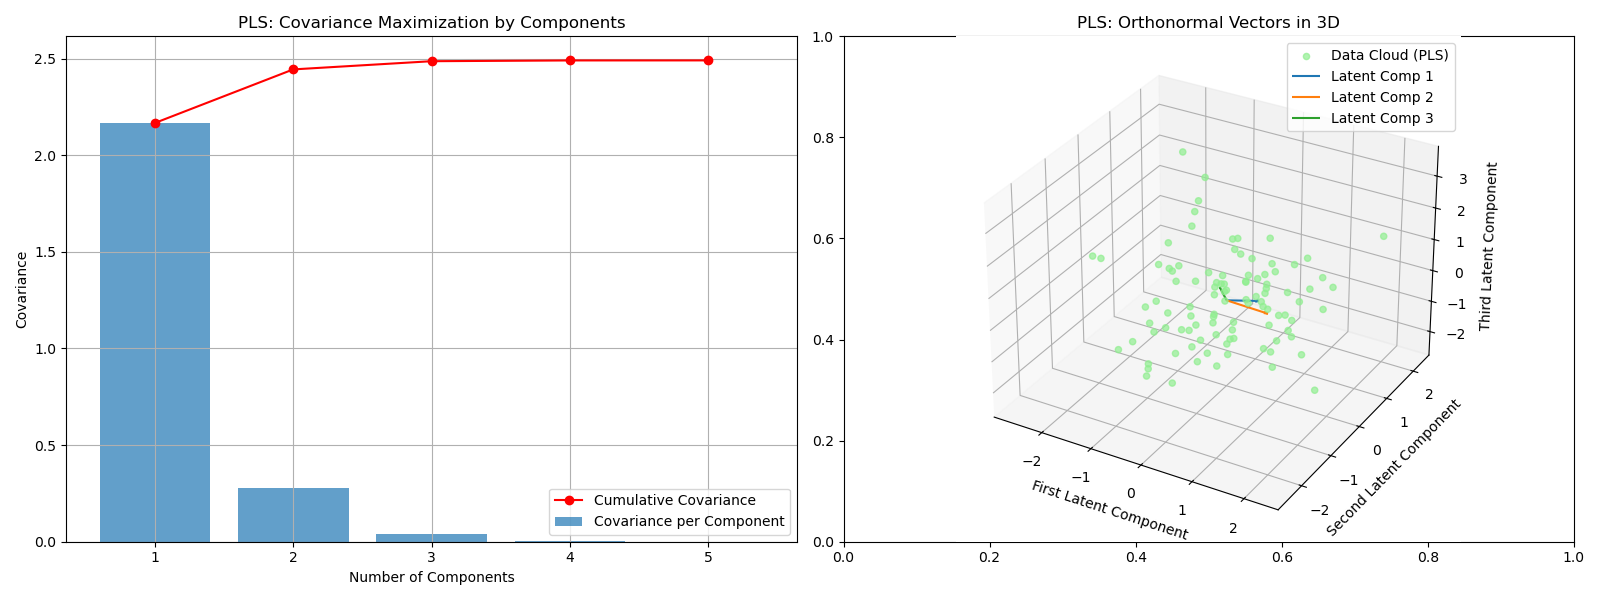
\includegraphics[width=0.9\textwidth]{PLS_Selected_Analysis.png}
    \caption{Partial Least Squares (PLS) Analysis Results}
    \label{fig:PLS_analysis}
\end{figure}



\subsection{Selection of the Optimal Number of Components in PCR and PLS}
A crucial aspect of applying PCR and PLS effectively is determining the appropriate number of components (\( k \)) to retain. Selecting too few components may result in underfitting, where important predictive information is lost. Conversely, retaining too many components can lead to overfitting, reducing the generalization ability of the model. Various methods are available to guide this selection:
\subsection{Elbow Method for PCR and PLS}
The Elbow Method is a widely used heuristic for selecting the optimal number of components in both Principal Component Regression (PCR) and Partial Least Squares (PLS). The method involves plotting a performance metric—such as cumulative explained variance for PCR or cumulative explained covariance for PLS—against the number of components. The optimal number of components is chosen at the "elbow point", where the marginal gain in variance or covariance explained diminishes significantly.

\subsubsection{Elbow Method for Principal Component Regression (PCR)}
In Principal Component Regression (PCR), component selection is based on Principal Component Analysis (PCA), which transforms the original predictor space into a set of orthogonal components that explain the variance in \( X \). Since PCR does not consider the response variable \( Y \) in component selection, it relies on the cumulative explained variance of the predictors.

Mathematically, the proportion of variance explained by the first \( k \) principal components is given by:
\begin{equation}
\text{Explained Variance}(k) = \frac{\sum_{i=1}^{k} \lambda_i}{\sum_{i=1}^{p} \lambda_i}
\end{equation}
where \( \lambda_i \) are the eigenvalues of the covariance matrix \( X^T X \), which correspond to the variances captured by each principal component.

The selection of \( k \) is determined by identifying the "elbow point" on the cumulative variance plot. This is the point where adding more components results in a negligible increase in explained variance. In practical applications, a commonly used threshold is:
\begin{equation}
\sum_{i=1}^{k} \lambda_i \geq 0.95 \sum_{i=1}^{p} \lambda_i
\end{equation}
indicating that at least 95\% of the total variance in \( X \) has been retained.

\subsubsection{Elbow Method for Partial Least Squares (PLS)}
Unlike PCR, which selects components based solely on variance in \( X \), Partial Least Squares (PLS) extracts components that maximize the covariance between \( X \) and \( Y \). Therefore, the Elbow Method in PLS is based on the cumulative explained covariance rather than variance.

For PLS, we define the cumulative explained covariance as:
\begin{equation}
\text{Explained Covariance}(k) = \frac{\sum_{i=1}^{k} \text{Cov}(t_i, y)^2}{\sum_{i=1}^{p} \text{Cov}(t_i, y)^2}
\end{equation}
where \( t_i \) are the latent variables obtained from PLS, which are linear combinations of the original predictors.

Similar to PCR, the "elbow point" is identified on the cumulative covariance plot, marking the point beyond which additional components contribute minimally to predictive power. The typical threshold for PLS component selection is:
\begin{equation}
\sum_{i=1}^{k} \text{Cov}(t_i, y)^2 \geq 0.90 \sum_{i=1}^{p} \text{Cov}(t_i, y)^2
\end{equation}
indicating that at least 90\% of the total covariance between \( X \) and \( Y \) is captured by the first \( k \) components.

\subsubsection{Interpretation and Practical Considerations}
The Elbow Method provides a simple yet effective means of selecting \( k \), but its effectiveness depends on the dataset. If the "elbow" is not clearly visible, alternative methods such as the \textbf{Needle Algorithm} or \textbf{Cross-Validation (CV)} should be used to refine component selection.

In summary:
- For PCR, components are selected based on explained variance, ensuring that the most important directions in \( X \) are retained.
- For PLS, components are selected based on explained covariance, ensuring that the most predictive directions for \( Y \) are retained.

A combination of these methods, along with domain knowledge, should guide the final selection of \( k \) to balance model complexity and predictive performance.

\subsubsection{Needle Algorithm for PCR and PLS}
The Needle Algorithm is an alternative method for determining the optimal number of components in Principal Component Regression (PCR) and Partial Least Squares (PLS). Unlike the Elbow Method, which relies on a visual inspection of a variance or covariance plot, the Needle Algorithm provides a formalized way of detecting the point beyond which additional components contribute negligibly to the model. It is particularly useful when the variance or covariance decay is gradual, making the elbow point ambiguous.

\paragraph{Needle Algorithm for Principal Component Regression (PCR)}
In Principal Component Regression (PCR), the goal is to select the number of components \( k \) that retain most of the variance in \( X \) while avoiding unnecessary complexity. The Needle Algorithm identifies \( k \) by examining the second derivative of the cumulative explained variance function.

Mathematically, the proportion of variance explained by the first \( k \) components is:
\begin{equation}
\text{Explained Variance}(k) = \frac{\sum_{i=1}^{k} \lambda_i}{\sum_{i=1}^{p} \lambda_i}
\end{equation}
where \( \lambda_i \) are the eigenvalues of \( X^T X \). 

The \textbf{Needle Criterion} is defined as:
\begin{equation}
\Delta_k = \lambda_k - \lambda_{k+1}
\end{equation}
\begin{equation}
\text{Relative Gain}(k) = \frac{\Delta_k}{\sum_{i=1}^{k} \lambda_i}
\end{equation}

The optimal \( k \) is determined when the relative gain in explained variance falls below a predefined threshold \( \epsilon \), typically around \( 1\% \):
\begin{equation}
\frac{\lambda_k - \lambda_{k+1}}{\sum_{i=1}^{k} \lambda_i} < \epsilon
\end{equation}
This ensures that additional components do not contribute meaningfully to variance retention.

\paragraph{Needle Algorithm for Partial Least Squares (PLS)}
For Partial Least Squares (PLS), the Needle Algorithm follows the same principle but is applied to the explained covariance between \( X \) and \( Y \) instead of variance in \( X \). 

The proportion of covariance explained by the first \( k \) components is given by:
\begin{equation}
\text{Explained Covariance}(k) = \frac{\sum_{i=1}^{k} \text{Cov}(t_i, y)^2}{\sum_{i=1}^{p} \text{Cov}(t_i, y)^2}
\end{equation}
where \( t_i \) are the latent variables extracted by PLS.

The Needle Criterion for PLS is:
\begin{equation}
\Delta_k = \text{Cov}(t_k, y)^2 - \text{Cov}(t_{k+1}, y)^2
\end{equation}
\begin{equation}
\text{Relative Gain}(k) = \frac{\Delta_k}{\sum_{i=1}^{k} \text{Cov}(t_i, y)^2}
\end{equation}

As in PCR, the optimal \( k \) is found when the relative gain in explained covariance drops below a predefined threshold \( \epsilon \):
\begin{equation}
\frac{\text{Cov}(t_k, y)^2 - \text{Cov}(t_{k+1}, y)^2}{\sum_{i=1}^{k} \text{Cov}(t_i, y)^2} < \epsilon
\end{equation}
Typically, \( \epsilon \) is set to 1\% to 2\%, ensuring that only significant components contributing to the prediction of \( Y \) are retained.

\subsubsection{Interpretation and Practical Considerations}
The Needle Algorithm provides a more formal alternative to the Elbow Method, particularly in cases where variance or covariance decays smoothly without a clear "elbow point." However:
\begin{itemize}
    \item \textbf{For PCR}, it helps determine the number of principal components that explain sufficient variance in \( X \).
    \item \textbf{For PLS}, it selects components based on their predictive power by maximizing the covariance between \( X \) and \( Y \).
    \item The threshold \( \epsilon \) should be chosen carefully to balance between model complexity and predictive accuracy.
\end{itemize}
A combination of methods, including the Elbow Method, Needle Algorithm, and Cross-Validation, is recommended to ensure an optimal choice of \( k \).
\subsubsection{Cross-Validation for PCR and PLS}
Cross-Validation (CV) is a data-driven approach to selecting the optimal number of components in Principal Component Regression (PCR) and Partial Least Squares (PLS). Unlike heuristic methods such as the Elbow Method or the Needle Algorithm, which focus on variance or covariance retention, CV directly evaluates the predictive performance of the model by minimizing the generalization error. This ensures that the selected number of components leads to the best tradeoff between bias and variance.

\paragraph{Cross-Validation for Principal Component Regression (PCR)}
In PCR, the key challenge is to determine how many principal components (\( k \)) should be retained to ensure strong predictive performance. Since PCR does not use the response variable \( Y \) when selecting components, cross-validation is crucial in identifying the point where including additional components no longer improves prediction accuracy.

The procedure for selecting \( k \) via CV follows these steps:
\begin{enumerate}
    \item Split the dataset into \( K \) \textbf{folds} (typically \( K = 5 \) or \( K = 10 \)).
    \item For each fold, fit the \textbf{PCR model} using the first \( k \) principal components and compute the prediction error on the held-out data.
    \item Compute the \textbf{Cross-Validation Mean Squared Error (CV-MSE)} for each \( k \):
    \begin{equation}
    \text{CV-MSE}(k) = \frac{1}{n} \sum_{i=1}^{n} (y_i - \hat{y}_{-i,k})^2
    \end{equation}
    where \( \hat{y}_{-i,k} \) is the prediction for the \( i \)-th observation using a model trained without that observation and with \( k \) components.
    \item Select \( k^* \) that minimizes \(\text{CV-MSE}(k)\):
    \begin{equation}
    k^* = \arg\min_k \text{CV-MSE}(k)
    \end{equation}
\end{enumerate}

Since PCR selects principal components without considering \( Y \), CV ensures that the selected components contribute to predictive accuracy rather than just maximizing variance in \( X \).

\paragraph{Cross-Validation for Partial Least Squares (PLS)}
Unlike PCR, where components are selected based only on variance in \( X \), PLS constructs components that maximize the covariance between \( X \) and \( Y \). Thus, CV in PLS plays a slightly different role: it helps determine the number of latent variables that maximize predictive accuracy.

The CV procedure for PLS follows the same general steps as in PCR:
\begin{enumerate}
    \item Split the dataset into \( K \) \textbf{folds}.
    \item For each fold, fit the \textbf{PLS model} using the first \( k \) latent variables and compute the prediction error on the held-out data.
    \item Compute the \textbf{CV-MSE} for each \( k \):
    \begin{equation}
    \text{CV-MSE}(k) = \frac{1}{n} \sum_{i=1}^{n} (y_i - \hat{y}_{-i,k})^2
    \end{equation}
    \item Select \( k^* \) that minimizes \(\text{CV-MSE}(k)\):
    \begin{equation}
    k^* = \arg\min_k \text{CV-MSE}(k)
    \end{equation}
\end{enumerate}

Since PLS incorporates \( Y \) in selecting components, it is expected to achieve lower CV-MSE compared to PCR for a given dataset, particularly when \( X \) and \( Y \) are highly correlated.

\subsubsection{Practical Considerations}
While cross-validation is the most rigorous method for selecting \( k \), it has some practical considerations:
\begin{itemize}
    \item \textbf{Computational Cost}: Cross-validation is computationally expensive since it requires training multiple models for different values of \( k \) across multiple folds.
    \item \textbf{Bias-Variance Tradeoff}: Smaller \( k \) values lead to higher bias, while larger \( k \) values lead to higher variance. CV helps find the optimal balance.
    \item \textbf{Choice of \( K \)}: Typically, \( K = 5 \) or \( K = 10 \) is used. A smaller \( K \) reduces computation time, but larger \( K \) provides a more reliable error estimate.
\end{itemize}

\subsubsection{Comparison of PCR and PLS using Cross-Validation}
\begin{itemize}
    \item \textbf{PCR} often requires more components than PLS to achieve the same predictive performance because it does not consider \( Y \) when selecting components.
    \item \textbf{PLS} typically achieves a lower optimal \( k^* \) due to its supervised nature, which aligns components with \( Y \).
    \item Both methods benefit from CV in avoiding overfitting by selecting an appropriate number of components.
\end{itemize}

\subsubsection{Final Recommendation}
Since CV provides a direct measure of predictive performance, it is considered the gold standard for selecting the number of components in both PCR and PLS, therefore CV is applied in our simulations and empirical estimation.

\subsubsection{Comparison of Methods}
\begin{itemize}
    \item The \textbf{Elbow Method} is computationally simple but may be subjective.
    \item The \textbf{Needle Algorithm} provides a more formal criterion but may still require expert judgment.
    \item \textbf{Cross-Validation} is the most robust, as it directly evaluates predictive performance, but it is computationally expensive.
\end{itemize}

\subsection{Final Thoughts on Component Selection}
The choice of \( k \) should be guided by a combination of these methods, balancing the need for variance retention and predictive accuracy. In empirical applications, cross-validation is typically preferred due to its ability to optimize for prediction error directly.
\newpage


\section{Simulation Study}

The goal of this simulation study is to evaluate the performance of Principal Component Regression (PCR) and Partial Least Squares (PLS) across different data-generating scenarios, focusing on their predictive accuracy, robustness, and bias-variance trade-offs in high-dimensional settings. Given the common challenges posed by multicollinearity and high-dimensional predictor spaces, we employ a Monte Carlo simulation framework to systematically analyze the behavior of these methods under varying feature dependencies. Simulation study is structured around three distinct setups:

\begin{enumerate}
    \item \textbf{Classical Data (No Multicollinearity)}: Predictors are independently sampled from a normal distribution, ensuring no multicollinearity.
    \item \textbf{Moderate Multicollinearity}: The predictor matrix consists of a set of base features along with additional highly correlated features, introducing a controlled level of dependence.
    \item \textbf{Severe Multicollinearity (Low Observations)}: The predictors exhibit strong correlations, with only a subset contributing to the response variable. This setup mimics scenarios where multicollinearity is extreme and sample size is limited, testing the methods' ability to extract meaningful structure from highly dependent data.
\end{enumerate}

To assess performance, we first apply PCR by performing Principal Component Analysis (PCA) on the predictor matrix and selecting the optimal number of components via \( k \)-fold cross-validation, minimizing the Root Mean Squared Error (RMSE) of prediction. Using these selected components, an Ordinary Least Squares (OLS) regression model is fitted, and predictive accuracy is evaluated through RMSE and Mean Squared Error (MSE). Additionally, we analyze the bias-variance trade-off of the coefficient estimates, comparing them to standard OLS results to quantify the extent of regularization. 

Similarly, for PLS, we employ the Nonlinear Iterative Partial Least Squares (NIPALS) algorithm to extract latent components, selecting the optimal number via cross-validation to balance model complexity and predictive power. A PLS regression model is then fitted to the transformed predictor matrix, with performance assessed through RMSE, MSE, and coefficient stability. 

To ensure the asymptotic validity of our findings, we conduct a Monte Carlo simulation, generating multiple datasets across the three setups to evaluate the stability of coefficient estimates, their bias-variance decomposition, and how these methods perform in large-sample scenarios. By systematically comparing PCR, PLS, and OLS across these conditions, we gain deeper insights into their relative advantages and limitations in high-dimensional regression problems.


\subsection{Data Description}
The dataset for each scenario is generated as follows:

\paragraph{Classical Data (No Multicollinearity)}
\begin{itemize}
    \item The predictor matrix \( X \) consists of \( n = 200 \) observations and \( p = 10 \) predictors, generated independently from a standard normal distribution:
    \[ X \sim \mathcal{N}(0, I_p) \]
    \item The response variable follows:
    \[ Y = X \beta + \epsilon, \quad \epsilon \sim \mathcal{N}(0, 0.1) \]
    \item All 10 predictors are actively used to generate \( Y \).
\end{itemize}

\paragraph{Moderate Multicollinearity}
\begin{itemize}
    \item The dataset contains \( n = 200 \) observations and \( p = 10 \) predictors.
    \item A \textbf{base predictor matrix} \( X_{\text{base}} \) is generated as:
    \[ X_{\text{base}} \sim \mathcal{N}(0, I) \]
    \item Additional features are constructed as:
    \[ X_{\text{extra}} = X_{\text{base}} + \eta, \quad \eta \sim \mathcal{N}(0, 0.1) \]
    where \( \eta \) introduces correlation between the predictors.
    \item The final predictor matrix is formed by concatenation:
    \[ X = [X_{\text{base}}, X_{\text{extra}}] \]
    \item The response variable is generated as:
    \[ Y = X \beta + \epsilon, \quad \epsilon \sim \mathcal{N}(0, 1.0) \]
    \item All 10 predictors are actively used to generate \( Y \).
\end{itemize}

\paragraph{Severe Multicollinearity (Low Observations)}
\begin{itemize}
    \item The dataset contains only \( n = 40 \) observations and \( p = 10 \) predictors, creating a scenario where the number of observations is significantly lower than in previous setups.
    \item A base predictor matrix is generated as:
    \[ X_{\text{gen}} \sim \mathcal{N}(0, I) \]
    \item Additional predictors are formed via a linear transformation:
    \[ X_{\text{additional}} = X_{\text{gen}} @ W + \mathcal{N}(0, 0.1) \]
    where \( W \) represents a randomly generated weight matrix, introducing strong collinearity among predictors.
    \item The response variable follows:
    \[ Y = X \beta + \epsilon, \quad \epsilon \sim \mathcal{N}(0, 1.0) \]
    \item Importantly, only \textbf{three} of the 10 predictors actively contribute to generating \( Y \), while the remaining seven are purely collinear noise variables.
\end{itemize}

In the severe multicollinearity scenario, the reduction in the number of observations relative to the number of predictors amplifies the risk of overfitting and instability in regression models. Furthermore, since only three predictors actively contribute to the response variable while the remaining seven are collinear noise, methods like PCR and PLS must effectively distinguish between relevant and redundant information. 

PCR, which selects components based on variance, may retain principal components influenced by multicollinear features, leading to potential inefficiencies in prediction. Conversely, PLS, which maximizes covariance with \( Y \), is expected to perform better in identifying relevant predictors, thus mitigating the negative impact of multicollinearity.

Each scenario is replicated 1000 times for statistical reliability.


\subsection{Simulation Results: Classical Dataset (No Multicollinearity)}  

In this scenario, the predictors are generated independently, ensuring there is no correlation between them. This setup creates the ideal conditions for Ordinary Least Squares (OLS) regression, which serves as the benchmark for evaluating Principal Component Regression (PCR) and Partial Least Squares (PLS). Our goal is to analyze how these methods perform when no multicollinearity is present and how their behavior changes as the number of components increases.

As expected, OLS performs the best, achieving the lowest Mean Squared Error (MSE) and producing coefficient estimates that closely match the true values. Because there is no multicollinearity, OLS remains unbiased and efficient, making it the optimal estimator in this setting. However, when we apply PCR and PLS, we see a clear difference in how they handle feature selection and regularization.  

\begin{figure}[H]
    \centering
    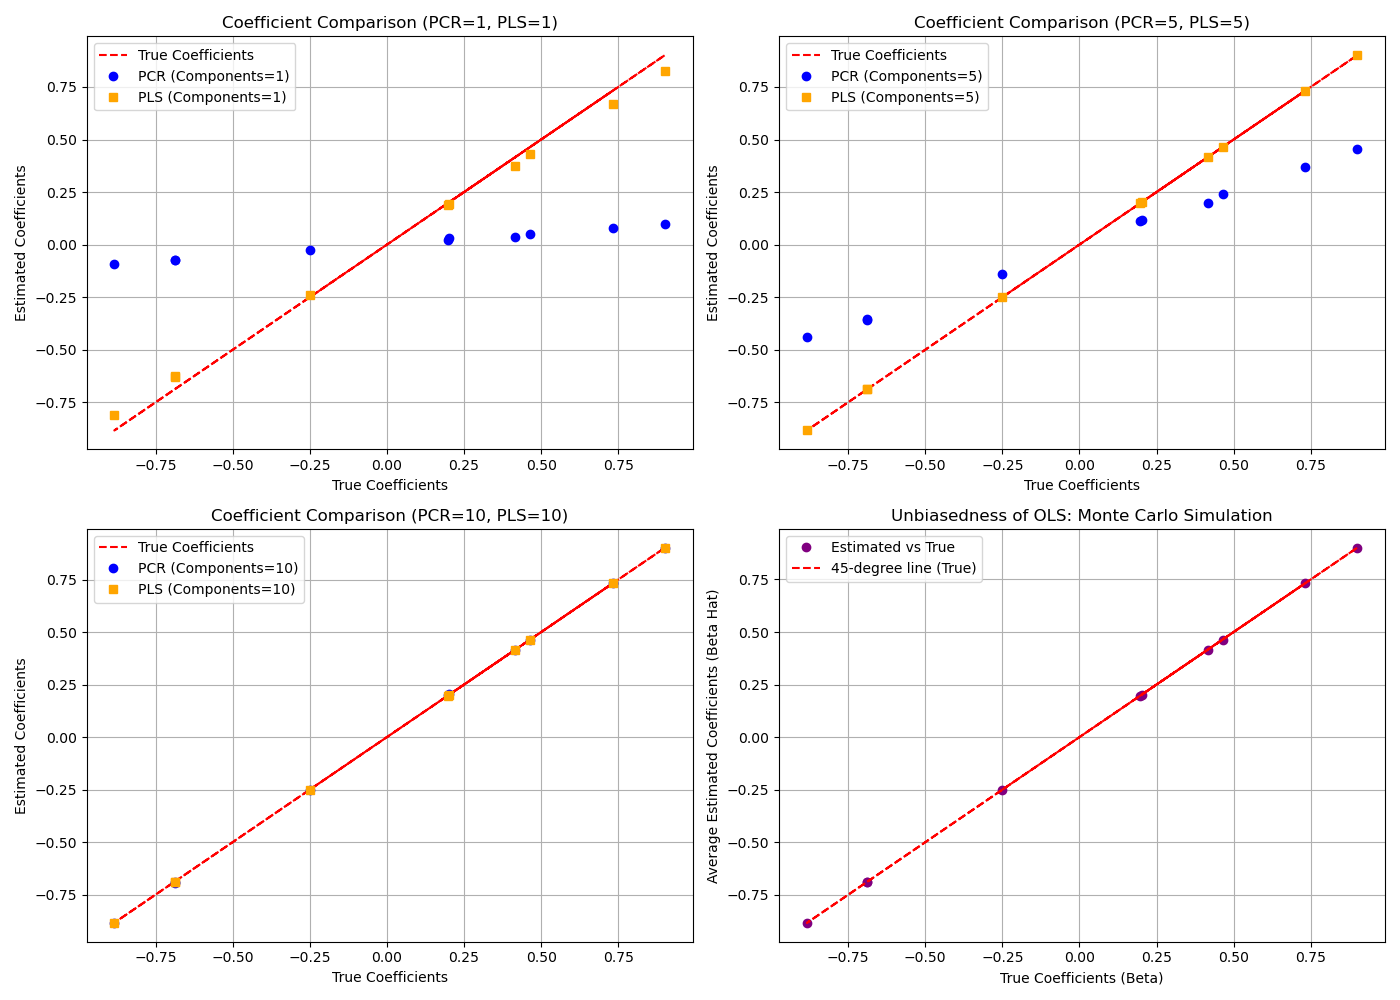
\includegraphics[width=0.9\textwidth]{First_plot.png}
    \caption{True vs Estimated coefficients: OLS, PCR and PLS}
    \label{fig:PLS_analysis}
\end{figure}

Since PCR selects components based purely on variance, it struggles when using only a few components. For instance, with PCR(1) (one principal component), the model captures only a limited portion of the predictor space, leading to high bias. However, as we increase the number of components (PCR(5), PCR(10)), the model recovers more information, reducing bias and approaching OLS-level accuracy. This improvement demonstrates the classic bias-variance trade-off: fewer components introduce higher bias but lower variance, while more components reduce bias at the cost of increasing variance.  


\begin{figure}[H]
    \centering
    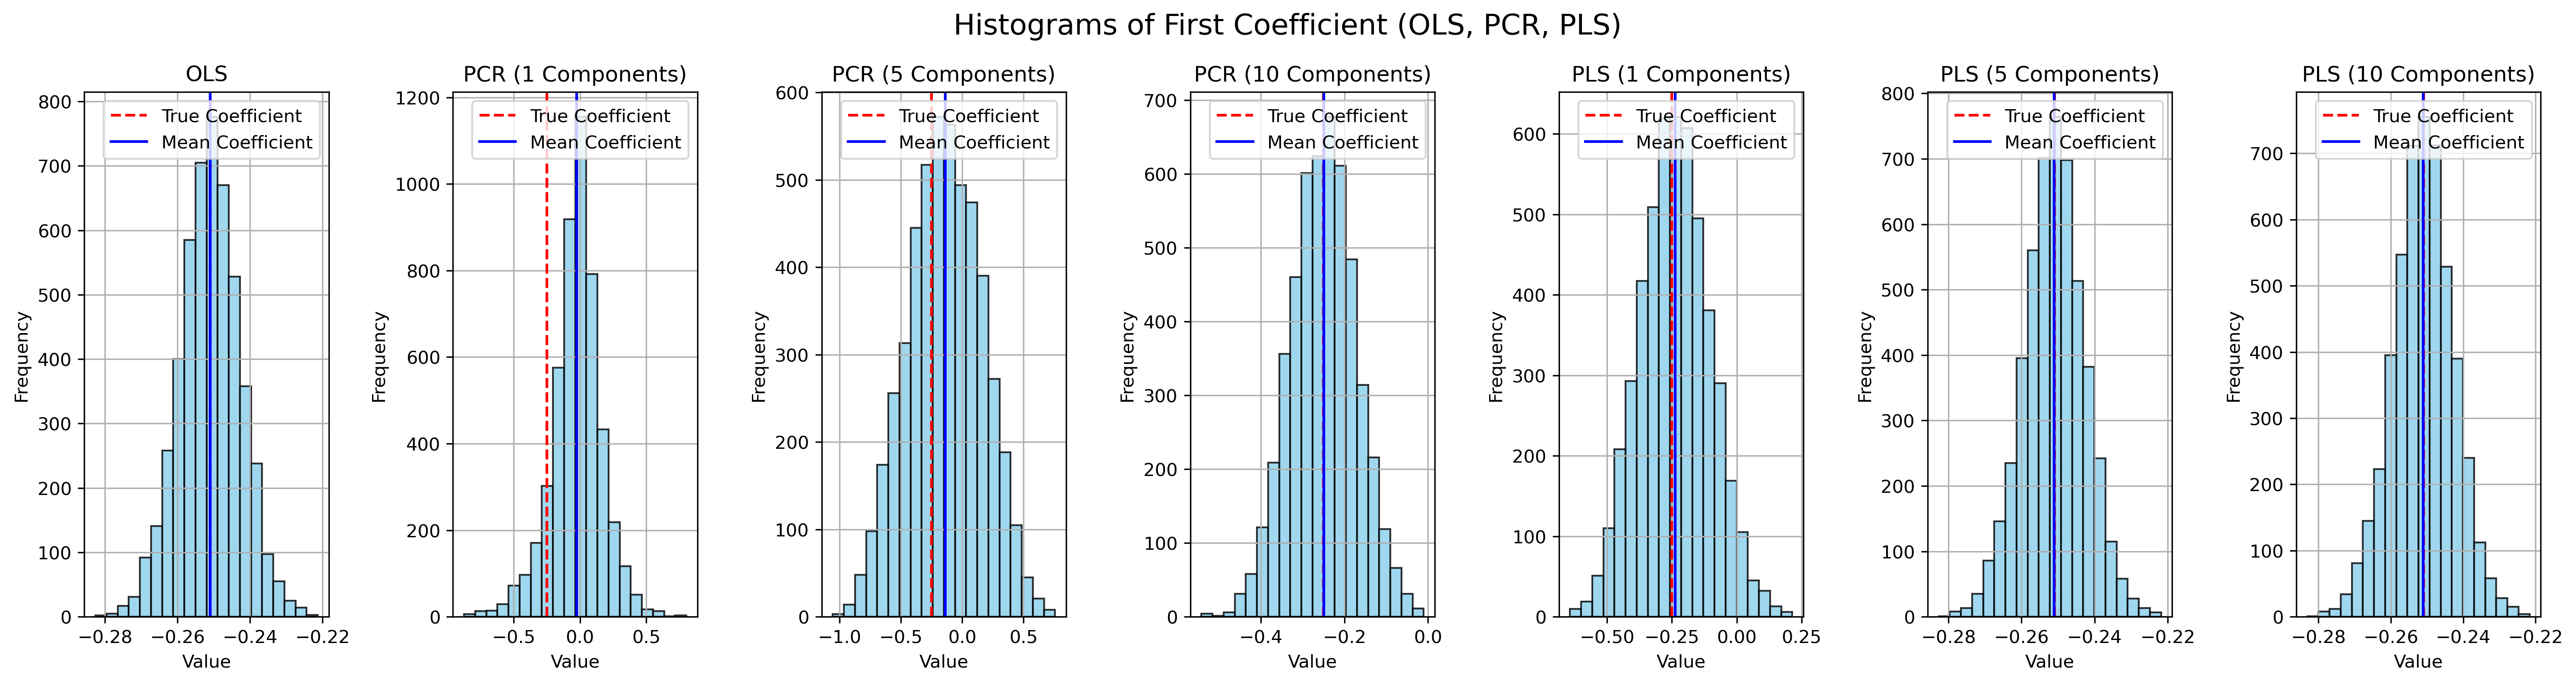
\includegraphics[width=0.9\textwidth]{Fourth_plot.png}
    \caption{Coefficient distribution: OLS, PCR and PLS}
    \label{fig:PLS_analysis}
\end{figure}

In contrast, PLS finds a balance between bias and variance more efficiently than PCR. Unlike PCR, which selects components based solely on predictor variance, PLS chooses components based on their relationship with the response variable. This allows PLS to extract relevant predictive features even with a small number of components. As a result, PLS with fewer components (e.g., PLS(1), PLS(5)) already provides better coefficient estimates and lower MSE compared to PCR with the same number of components. This suggests that PLS is a more efficient dimensionality reduction method when the goal is to improve prediction accuracy.

\begin{figure}[H]
    \centering
    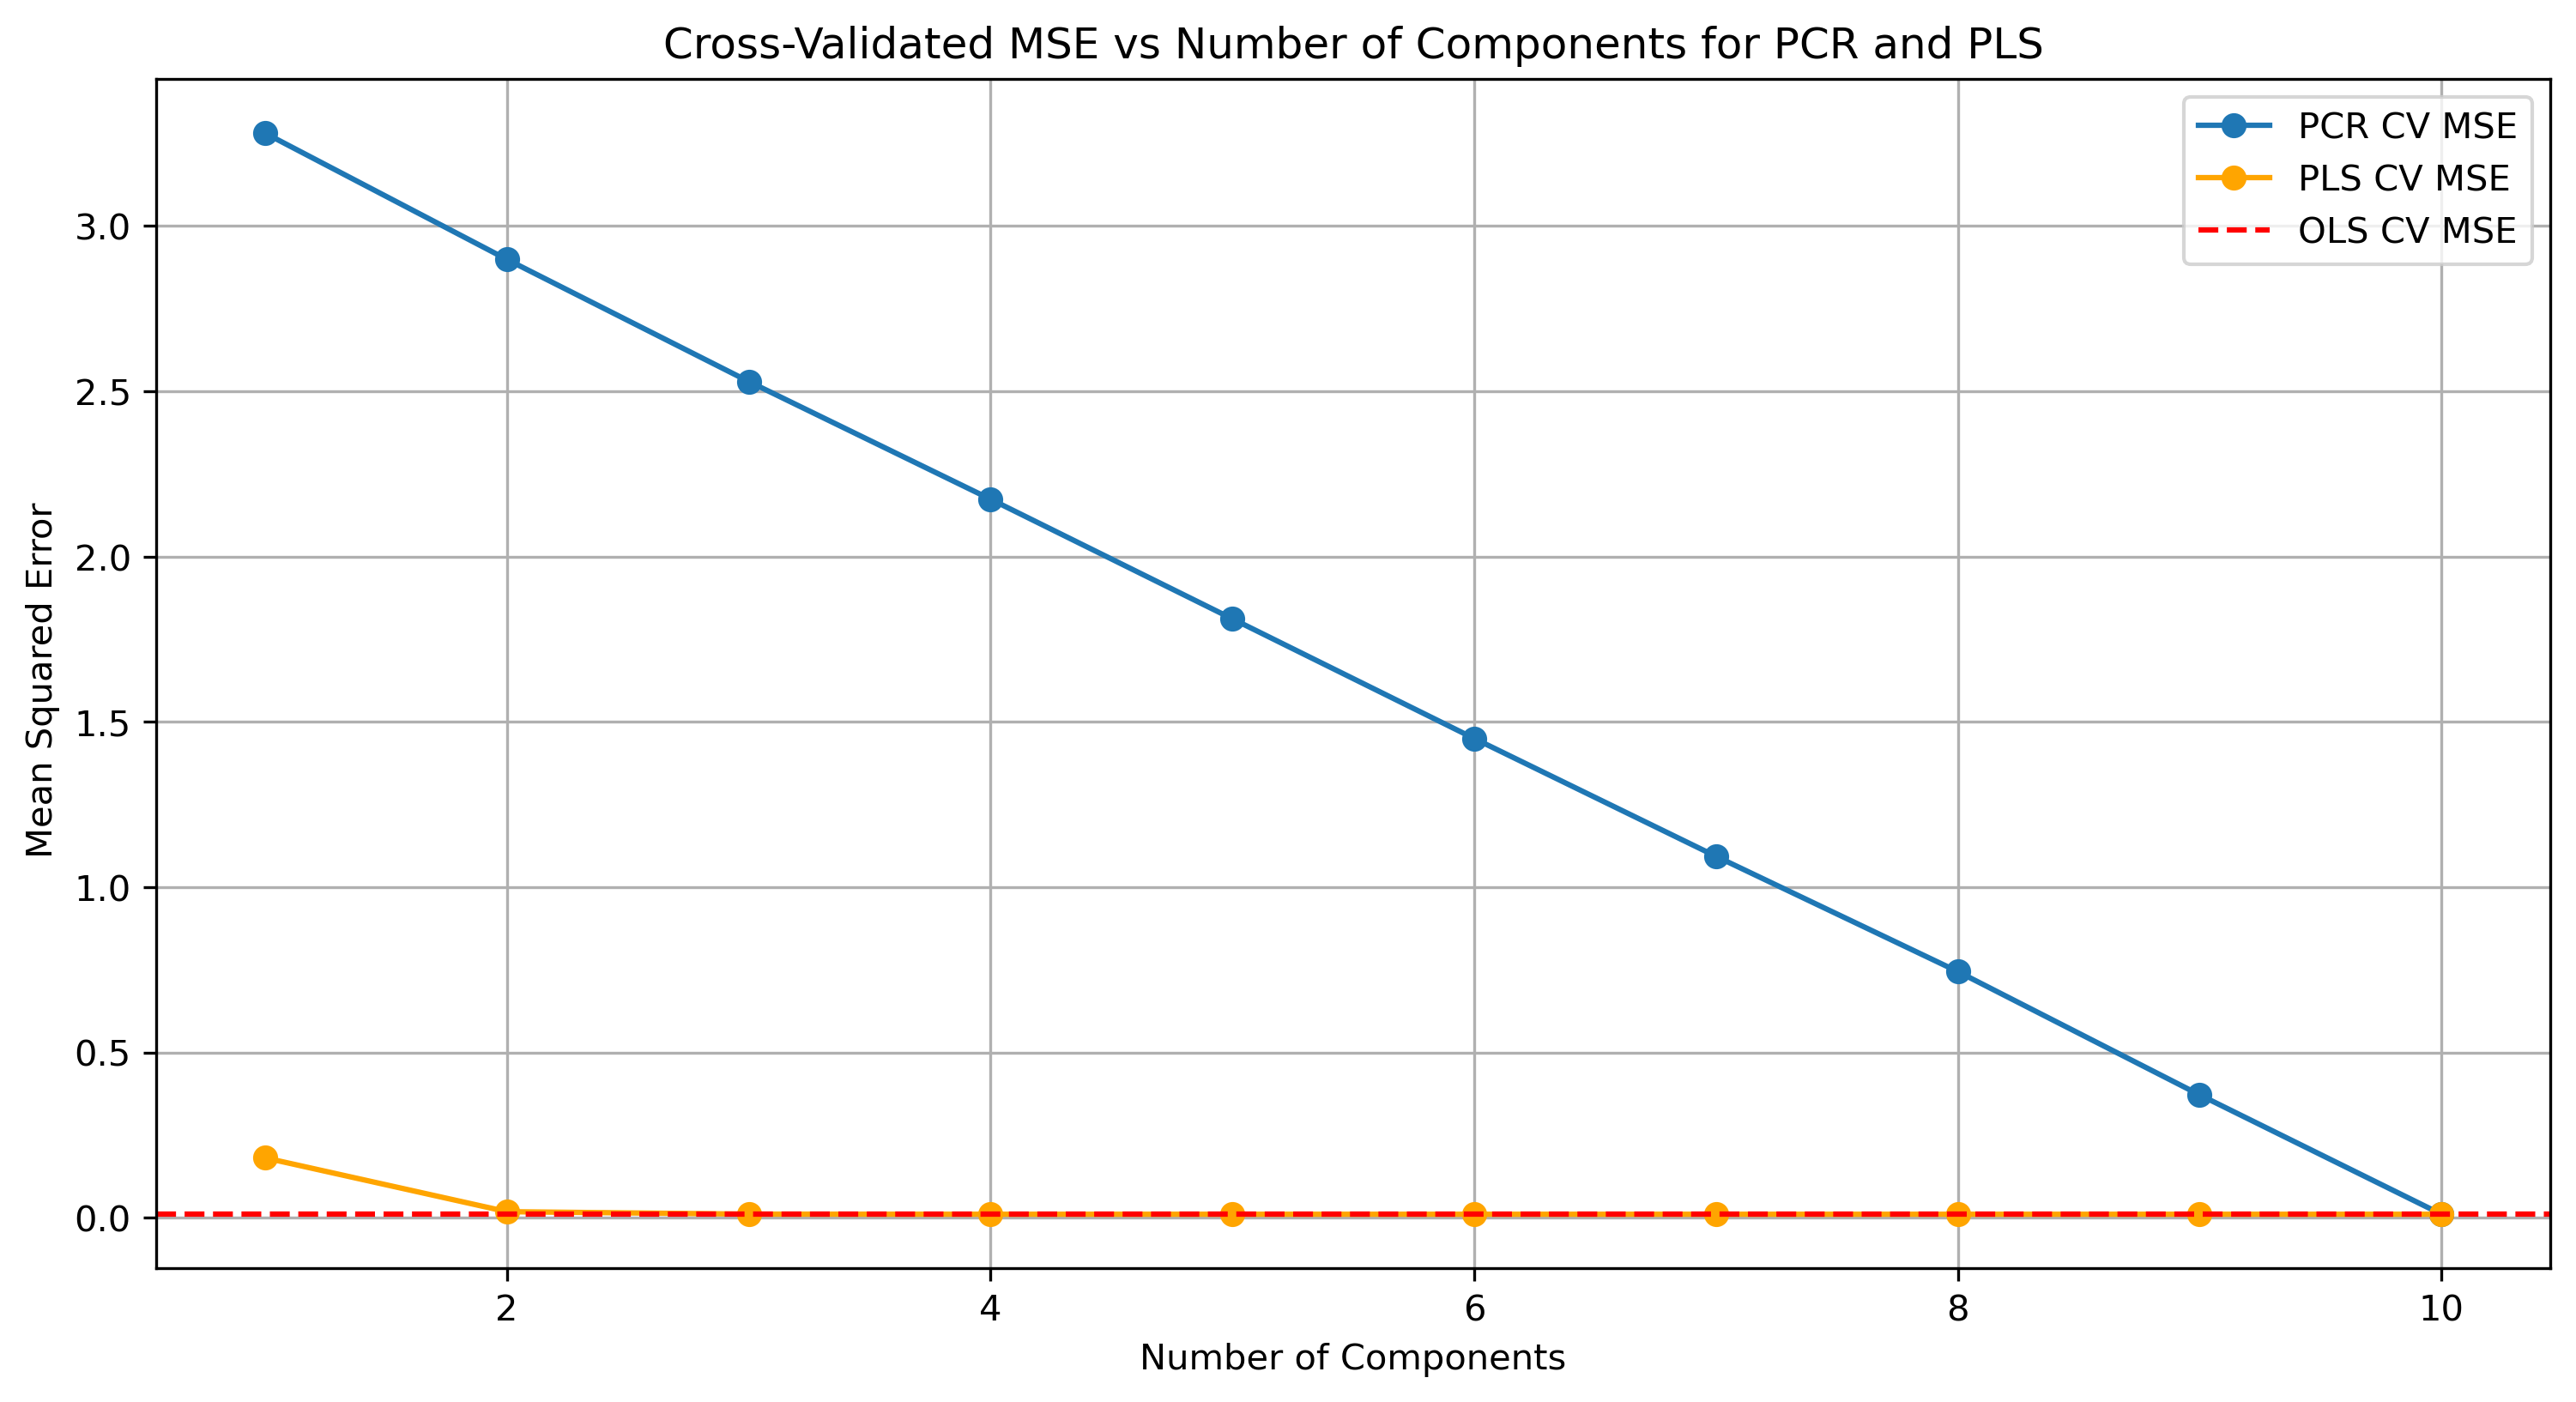
\includegraphics[width=0.9\textwidth]{Second_plot.png}
    \caption{CV MSE by components: OLS, PCR and PLS}
    \label{fig:PLS_analysis}
\end{figure}

The impact of component selection is further reflected in the quality of predictions. OLS predictions align almost perfectly with real values, reinforcing its reliability in this scenario. On the other hand, PCR with very few components, such as PCR(1), struggles to capture the full structure of the data, leading to poor predictions and a weaker fit. However, as the number of components increases, the predictions improve significantly, with PCR(10) closely matching the performance of OLS. In comparison, PLS consistently performs well even with fewer components, confirming its ability to extract meaningful features efficiently. This efficiency allows PLS to achieve strong predictive performance while using fewer dimensions than PCR, making it a more robust choice when dimensionality reduction is necessary.

The stability of coefficient estimates also reflects these patterns. OLS estimates remain centered around the true values with minimal variation, confirming that it is an unbiased estimator. PCR, on the other hand, shows greater variability when fewer components are used, and its estimates are further from the true values. However, when enough components are included, PCR estimates stabilize and align with OLS. PLS estimates remain more stable than PCR, even with fewer components, highlighting its advantage in capturing relevant information effectively.

\begin{figure}[H]
    \centering
    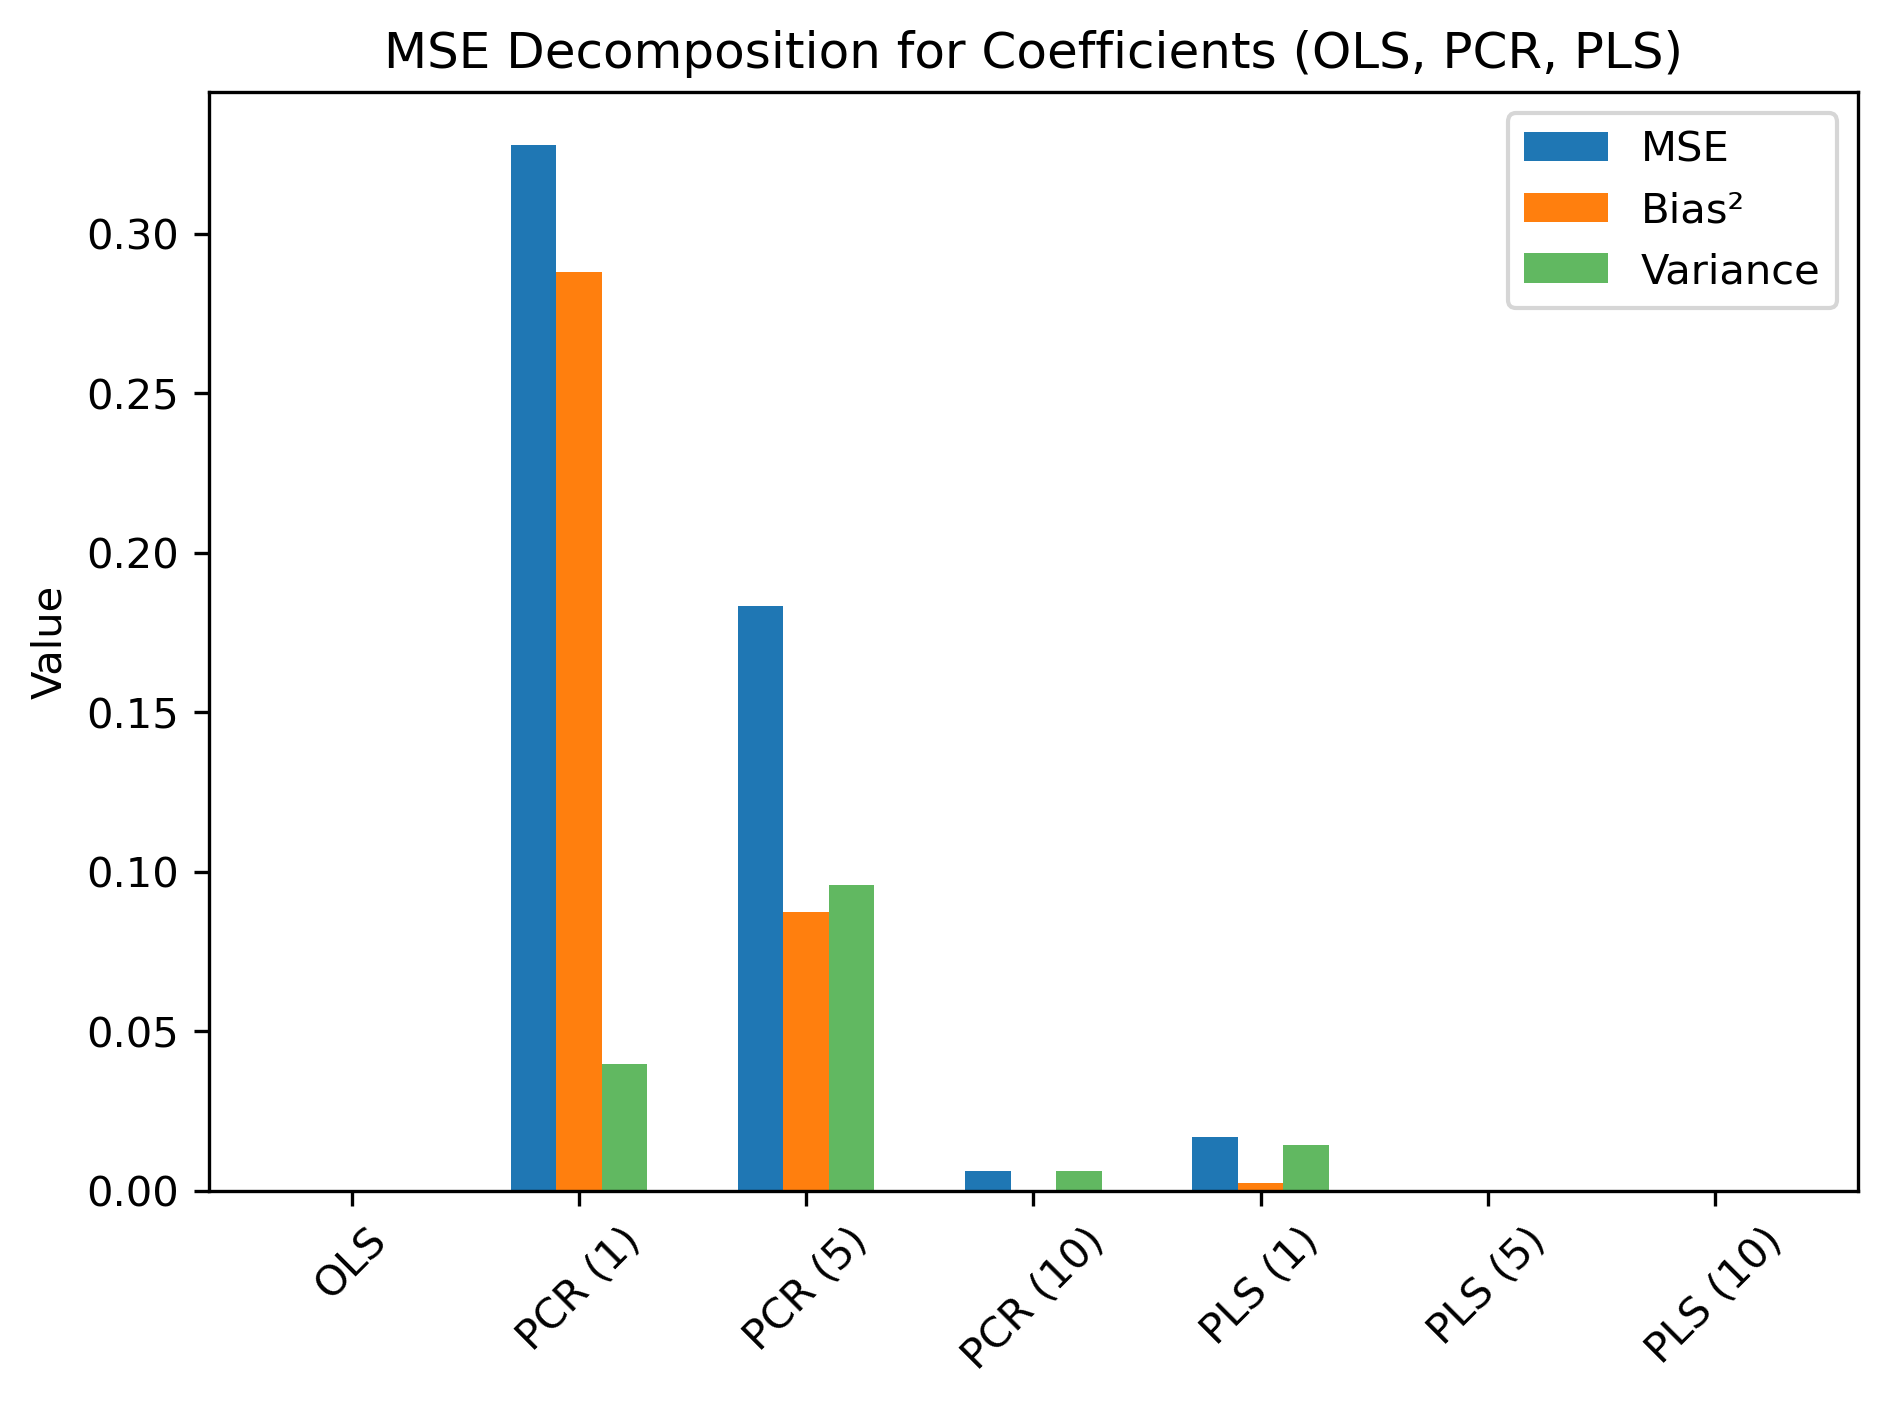
\includegraphics[width=0.9\textwidth]{Fifth_plot.png}
    \caption{Bias-Variance trade-off: OLS, PCR and PLS}
    \label{fig:PLS_analysis}
\end{figure}

OLS is the best option when there is no multicollinearity, as it provides the most accurate and stable coefficient estimates. PCR requires a sufficient number of components to recover the full predictor space. Using too few components results in high bias and poor predictions, but increasing the number of components improves performance. PLS is more efficient than PCR in selecting relevant features, achieving strong predictive performance with fewer components. The bias-variance trade-off is evident—fewer components lead to high bias (underfitting), while using too many components increases variance (potential overfitting).

\begin{figure}[H]
    \centering
    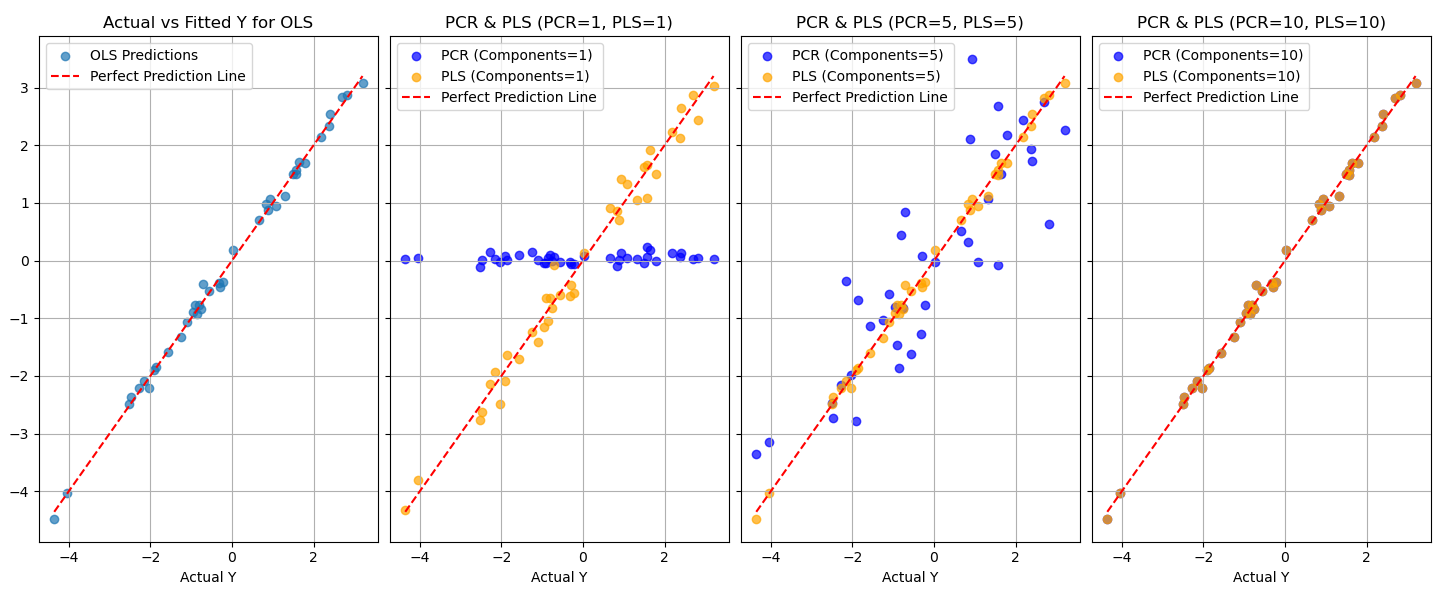
\includegraphics[width=0.9\textwidth]{Third_plot.png}
    \caption{Model fit: OLS, PCR and PLS}
    \label{fig:PLS_analysis}
\end{figure}

This classical dataset serves as a baseline reference, showing how PCR and PLS behave under ideal conditions. The next step is to explore how these methods perform when moderate multicollinearity is introduced, where predictors become correlated and the assumptions of OLS begin to break down.


\subsection{Simulation Results: Moderate Multicollinearity Dataset}  

In this scenario, the predictor variables are moderately correlated, introducing a controlled level of multicollinearity. This setup challenges the assumptions of Ordinary Least Squares (OLS) regression and allows us to assess how Principal Component Regression (PCR) and Partial Least Squares (PLS) handle collinearity and improve prediction performance.

When predictors exhibit moderate multicollinearity, OLS starts to struggle as the variance of coefficient estimates increases. This is evident in the Mean Squared Error (MSE) decomposition, where OLS has a significantly high variance component. While OLS remains unbiased, its estimates become unstable due to the correlated predictors.

\begin{figure}[H]
    \centering
    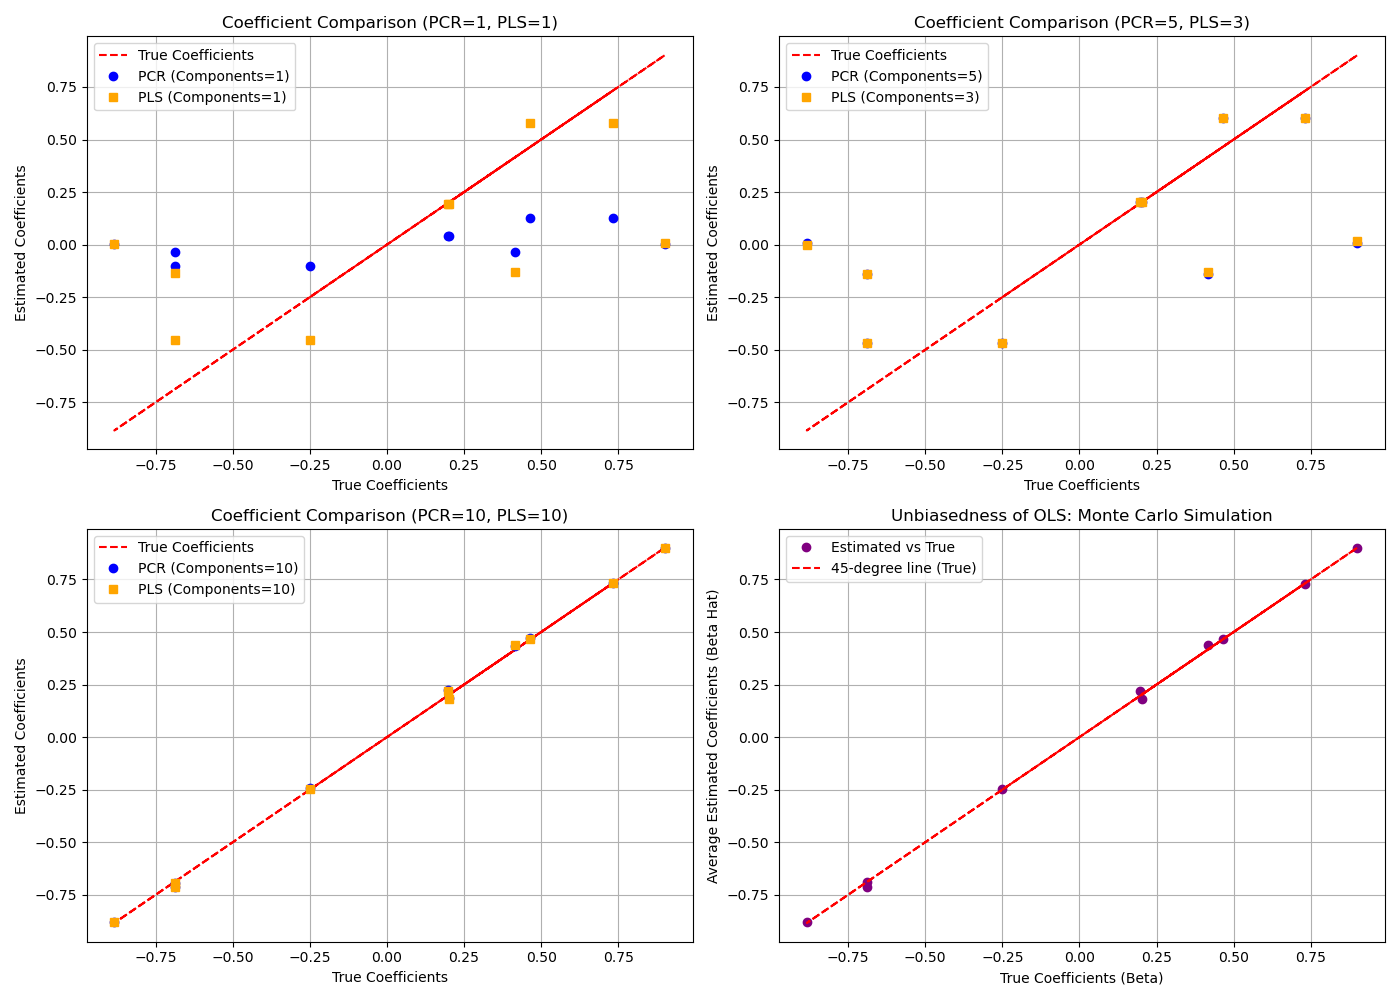
\includegraphics[width=0.9\textwidth]{First_plot_second_simulation.png}
    \caption{True vs Estimated coefficients: OLS, PCR and PLS}
    \label{fig:PLS_analysis}
\end{figure}

PCR mitigates this issue by reducing the predictor space to uncorrelated principal components. However, with too few components (e.g., PCR(1)), the model captures only limited variance, resulting in high bias. As the number of components increases (PCR(5), PCR(10)), bias decreases, and the model performance improves. Nevertheless, PCR does not explicitly use response variable information when selecting components, which can lead to inefficiencies in retaining relevant predictive information.

\begin{figure}[H]
    \centering
    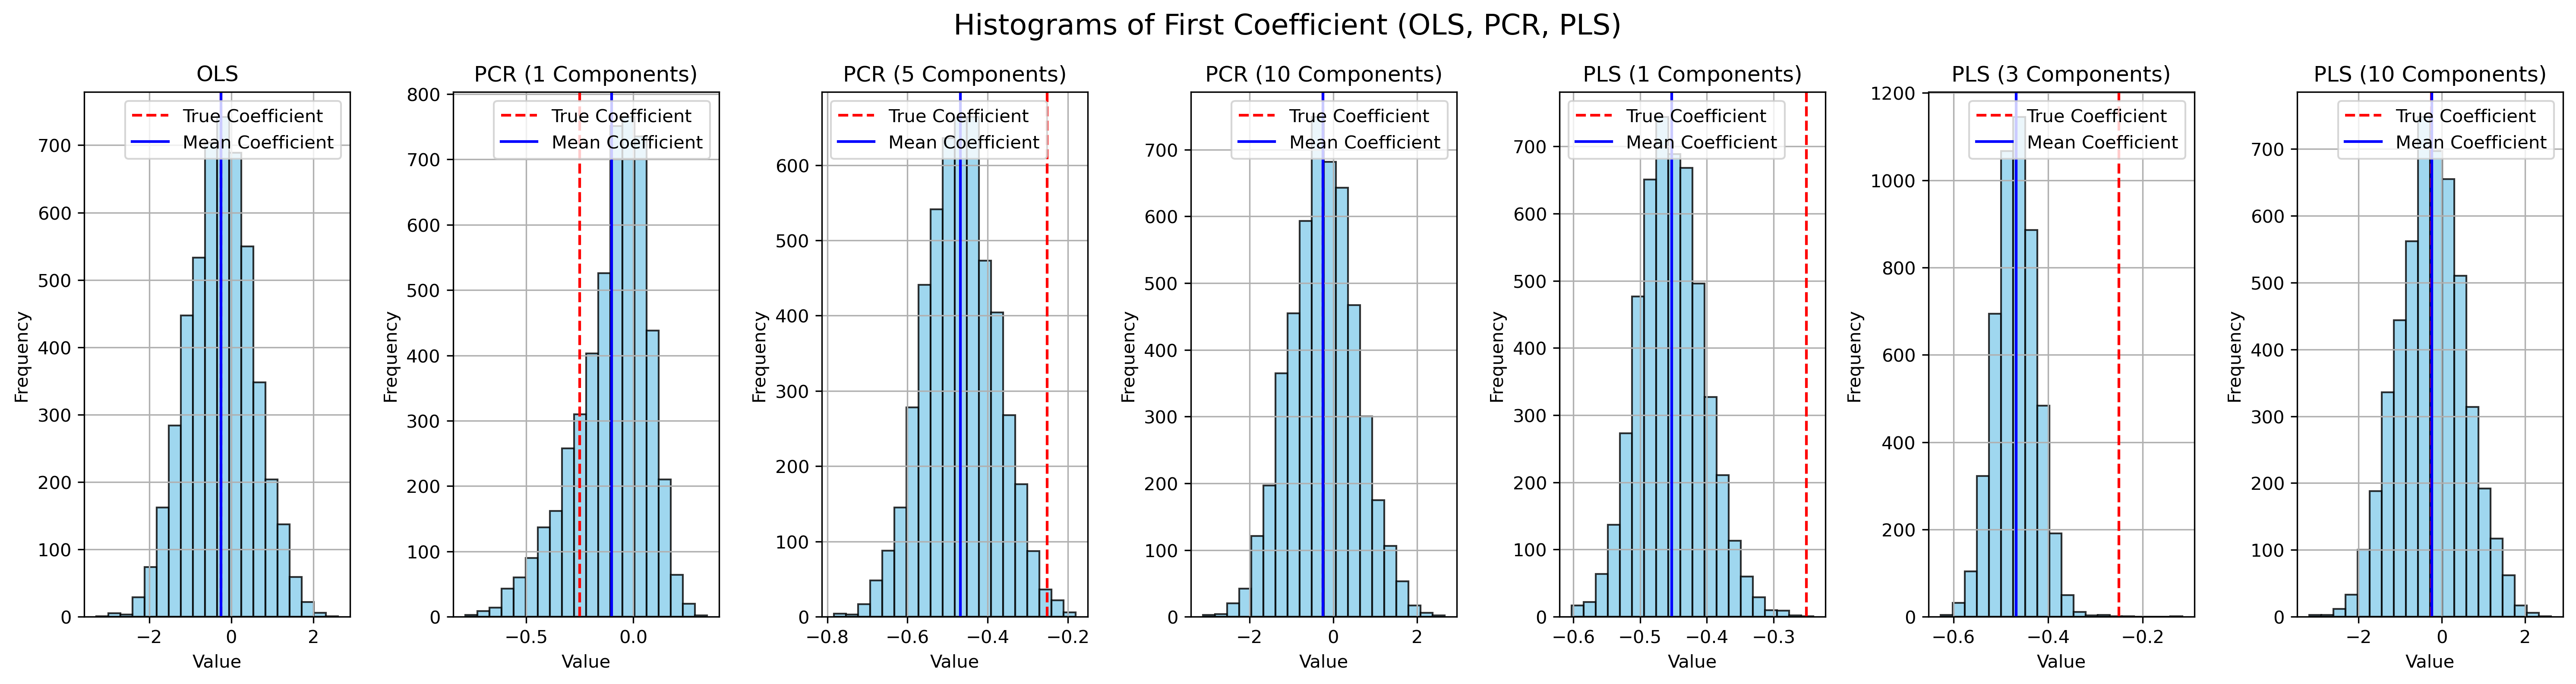
\includegraphics[width=0.9\textwidth]{Fourth_plot_second_simulation.png}
    \caption{Coefficient distribution: OLS, PCR and PLS}
    \label{fig:PLS_analysis}
\end{figure}

PLS, in contrast, is designed to extract components that maximize covariance with the response variable. This allows PLS to achieve a better balance between bias and variance with fewer components compared to PCR. Even with a small number of components (e.g., PLS(3)), it outperforms PCR with the same number of components, as it better identifies the underlying structure in the data.

The impact of multicollinearity on model predictions becomes evident when comparing actual vs. predicted values. OLS predictions are less stable due to inflated coefficient variance, leading to fluctuations in its predictive performance. PCR with very few components underfits the data, failing to capture enough variance for accurate predictions. However, as the number of components increases, PCR’s predictions align more closely with actual values, though it still lags behind PLS.

PLS consistently provides a stronger predictive fit, even with fewer components. Its predictions are closer to the true values, demonstrating that selecting components based on their relevance to the response variable improves generalization. This makes PLS a more robust choice when multicollinearity is present.

\begin{figure}[H]
    \centering
    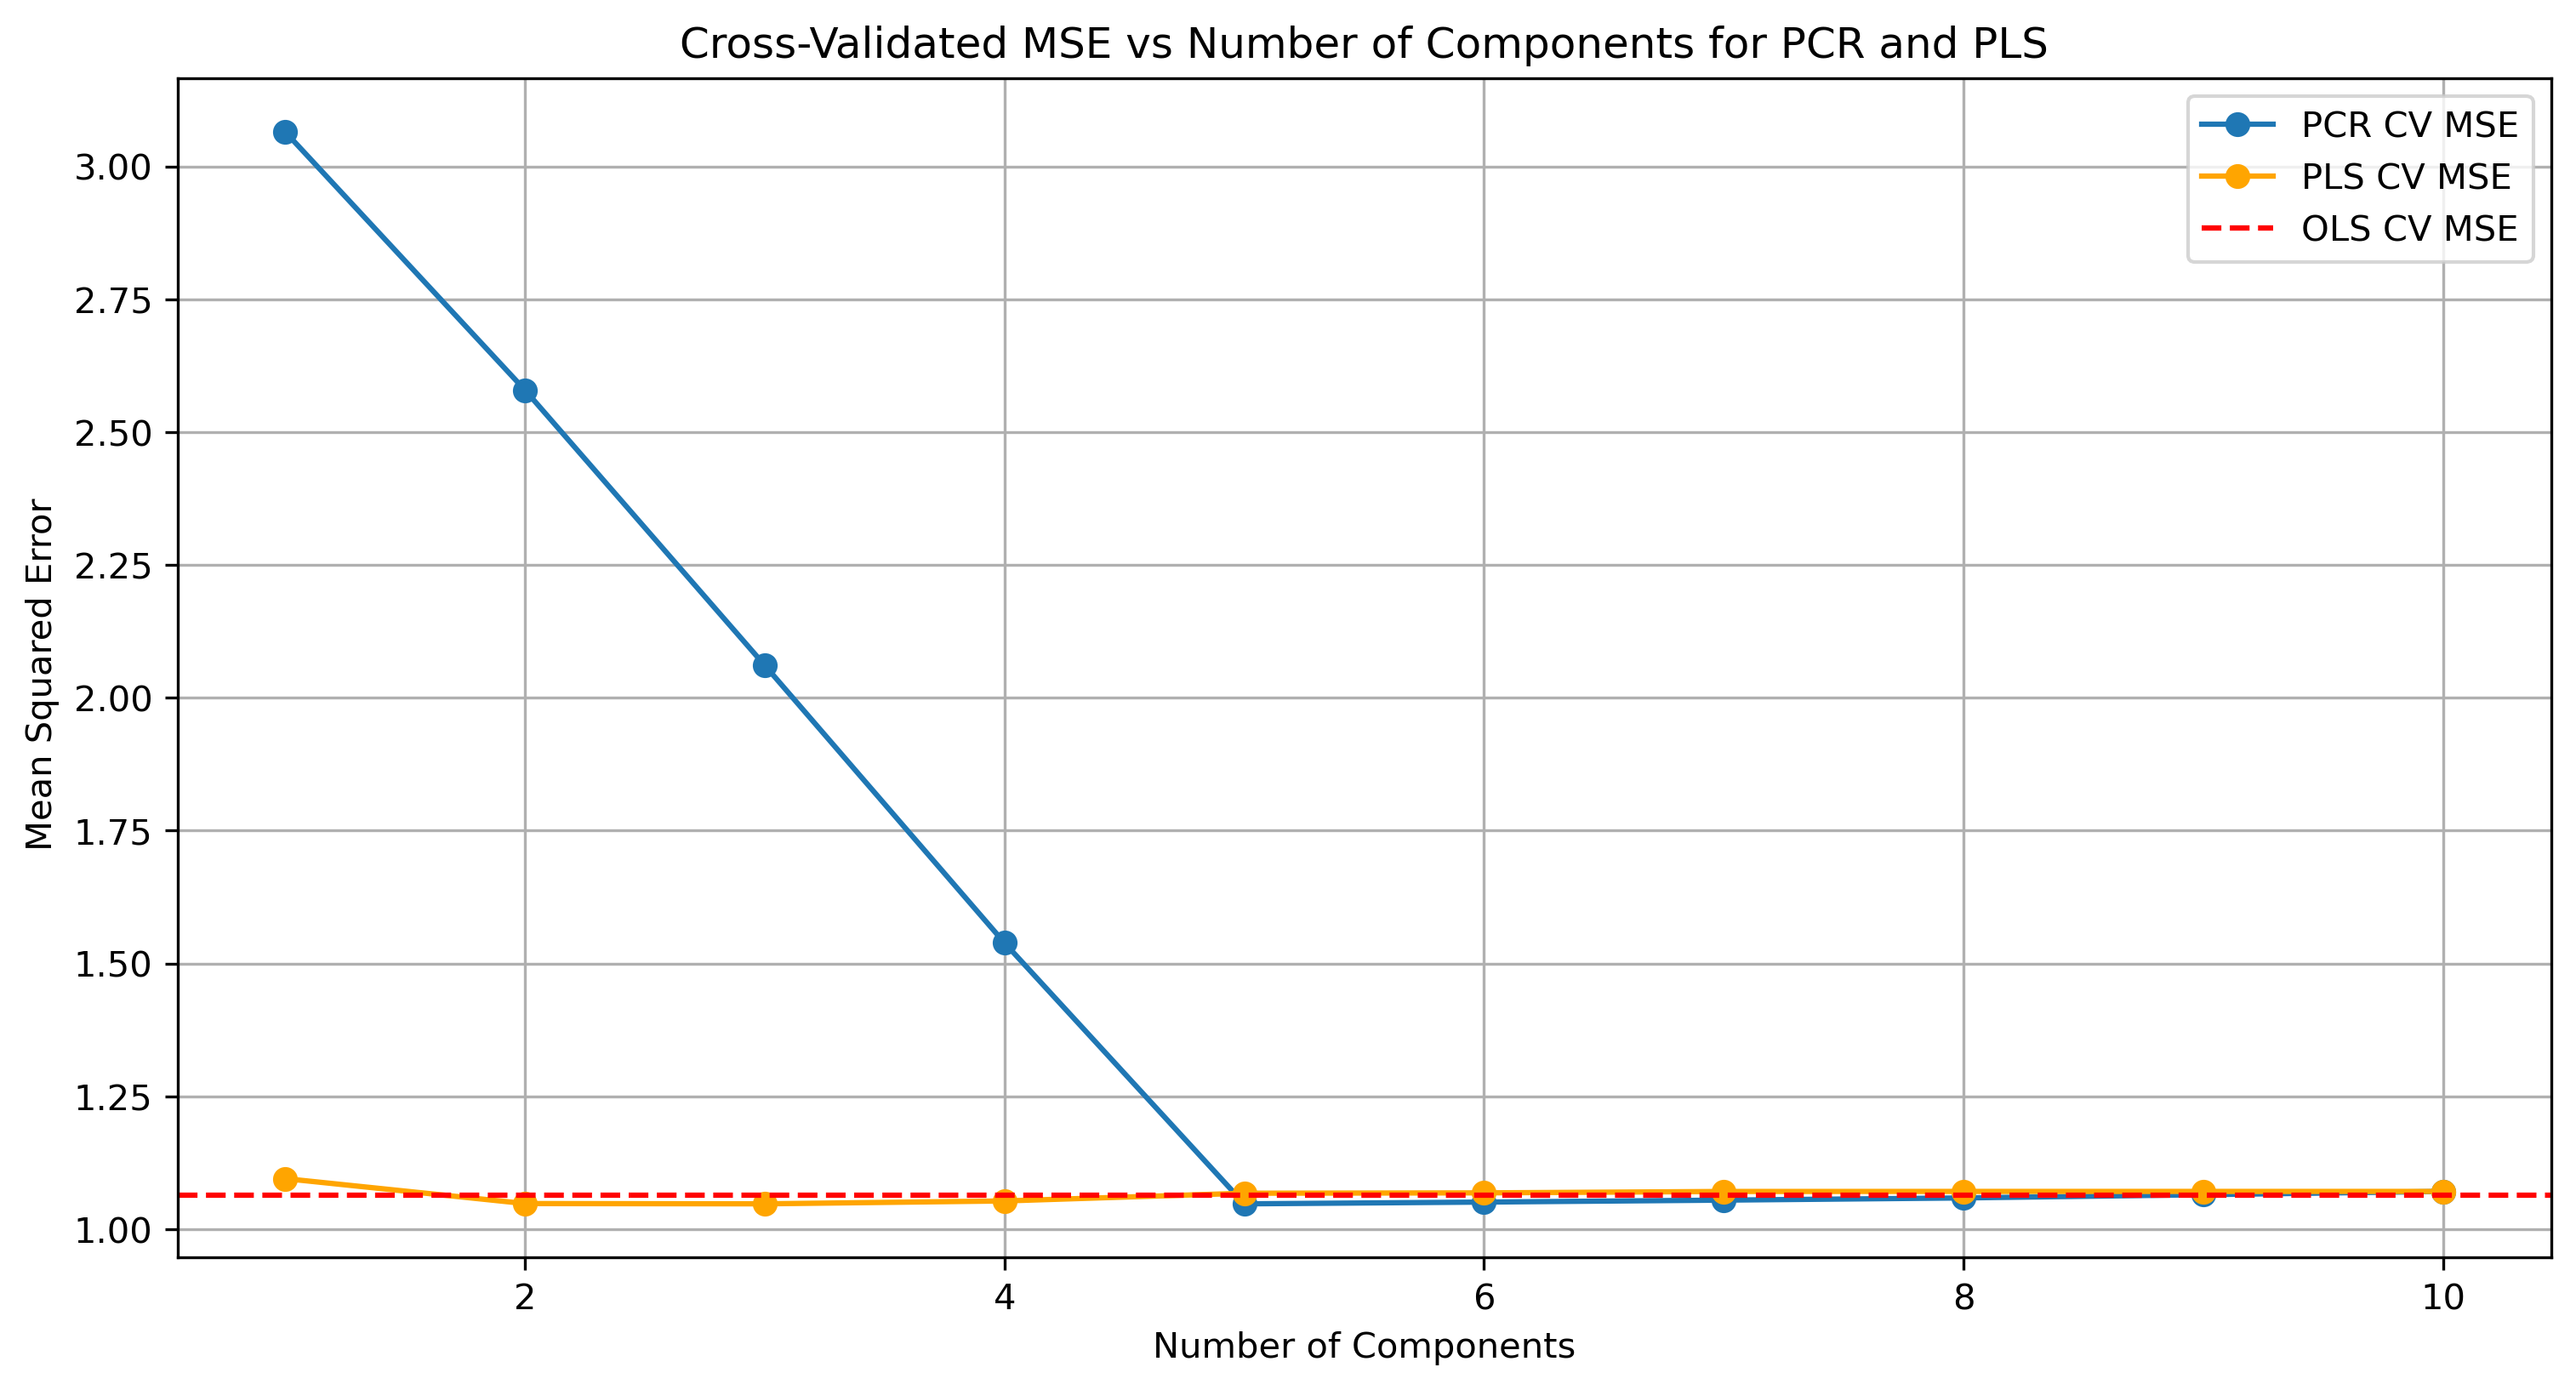
\includegraphics[width=0.9\textwidth]{Second_plot_second_simulation.png}
    \caption{CV MSE by components: OLS, PCR and PLS}
    \label{fig:PLS_analysis}
\end{figure}

The stability of coefficient estimates also reflects these patterns. OLS estimates show high variability, confirming its sensitivity to multicollinearity. PCR, when using too few components, exhibits significant bias, whereas with more components, its estimates stabilize. PLS remains more stable than PCR throughout, highlighting its effectiveness in handling multicollinearity.


\begin{figure}[H]
    \centering
    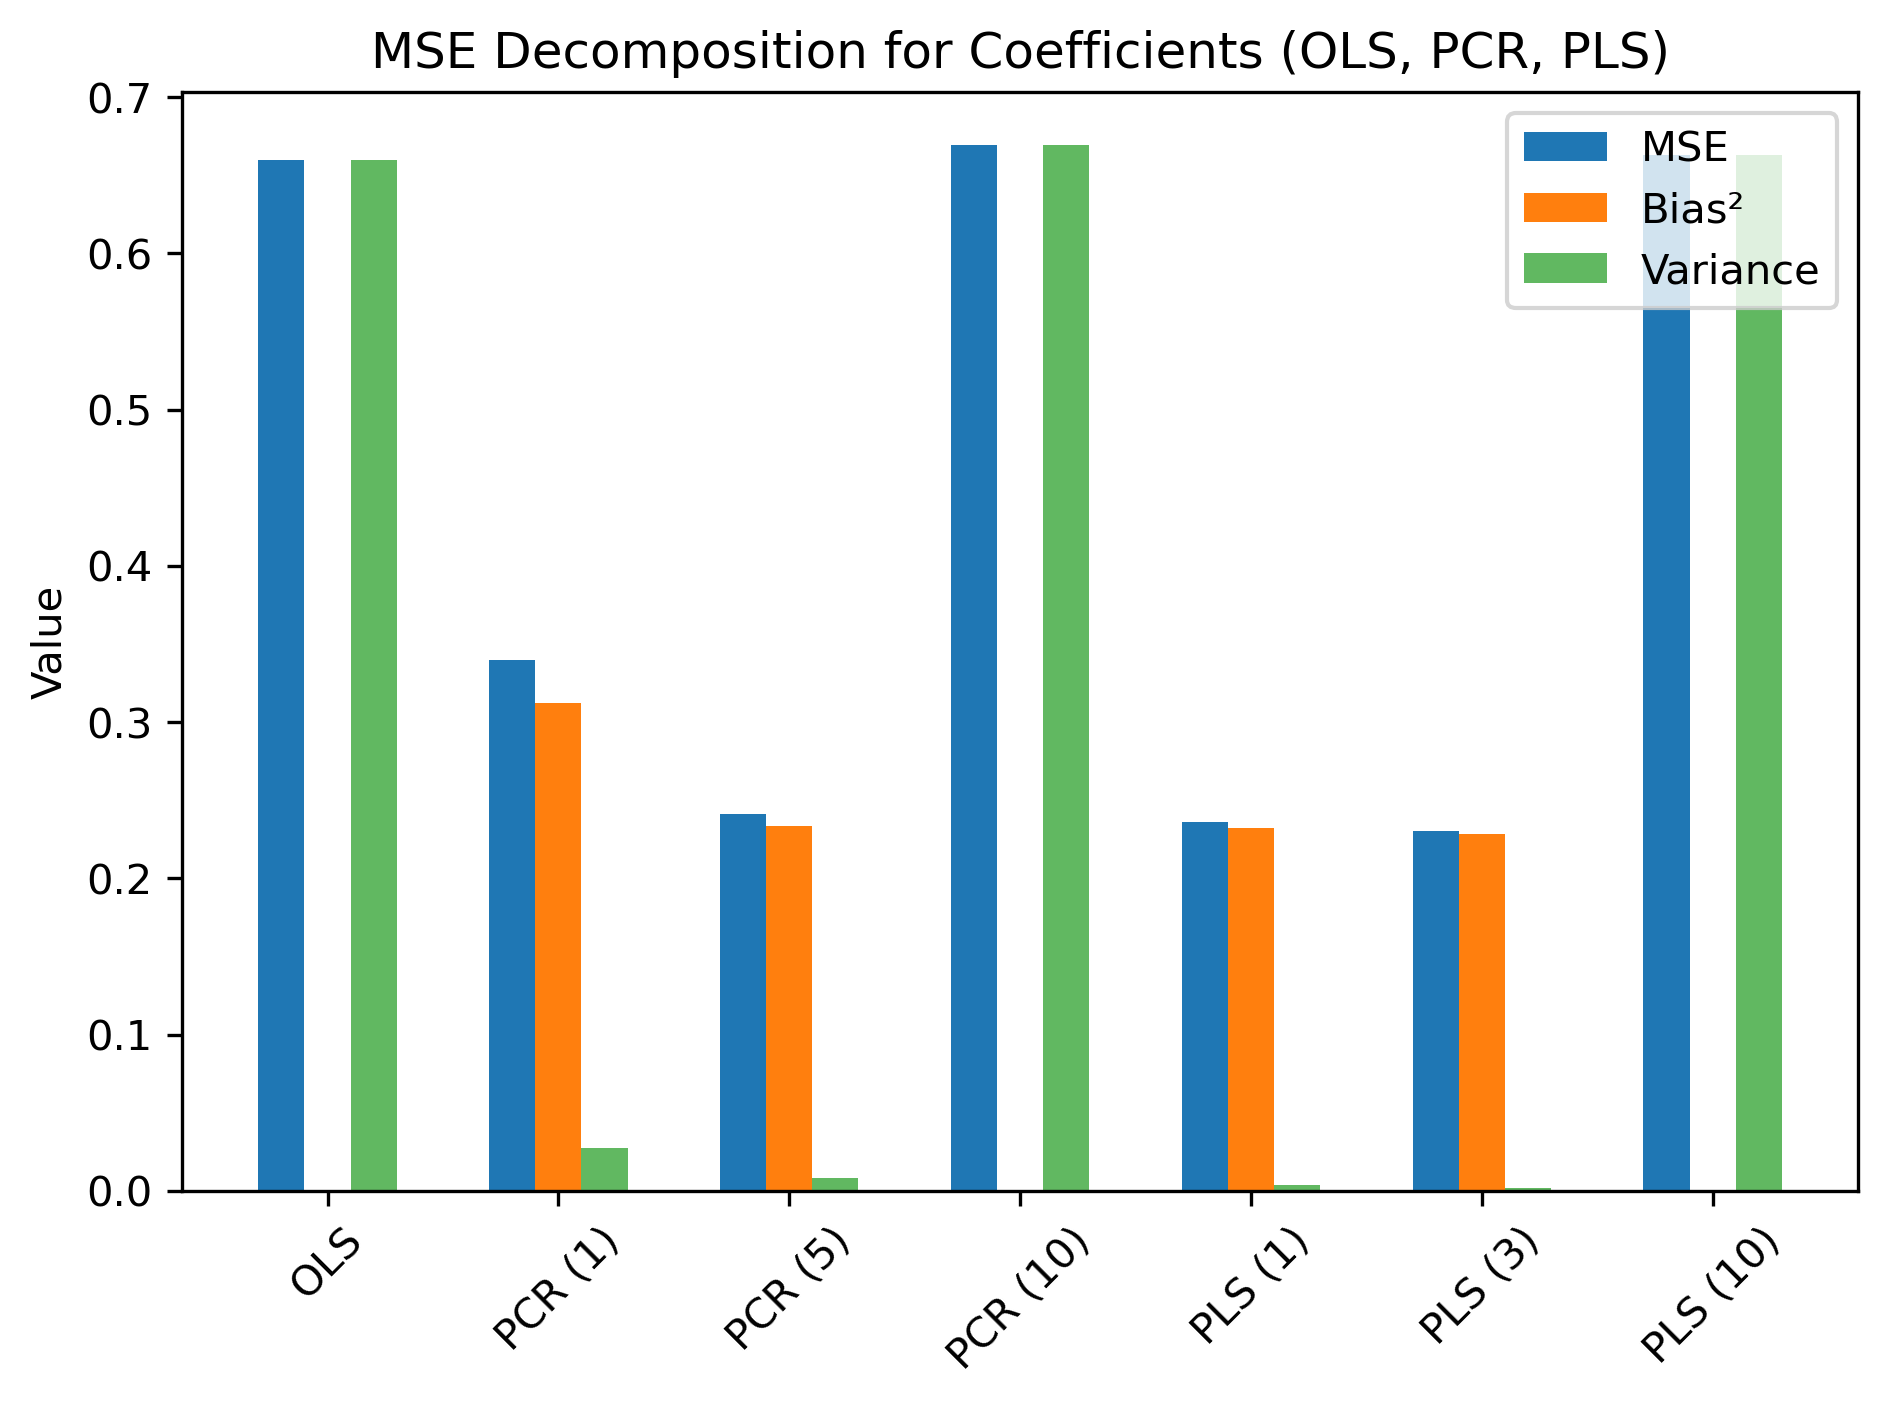
\includegraphics[width=0.9\textwidth]{Fifth_plot_second_simulation.png}
    \caption{Bias-Variance trade-off: OLS, PCR and PLS}
    \label{fig:PLS_analysis}
\end{figure}

OLS struggles in the presence of moderate multicollinearity, with high variance in coefficient estimates reducing prediction stability. PCR mitigates multicollinearity but requires enough components to recover essential variance. Selecting too few components results in high bias, while increasing components gradually improves predictions. PLS effectively balances bias and variance, leveraging response-driven component selection to achieve strong predictive performance with fewer components. PLS outperforms PCR in handling multicollinearity, as it selects components that are directly relevant to the response variable rather than relying solely on variance. The bias-variance trade-off remains crucial—too few components lead to underfitting (high bias), whereas too many components can introduce instability.

\begin{figure}[H]
    \centering
    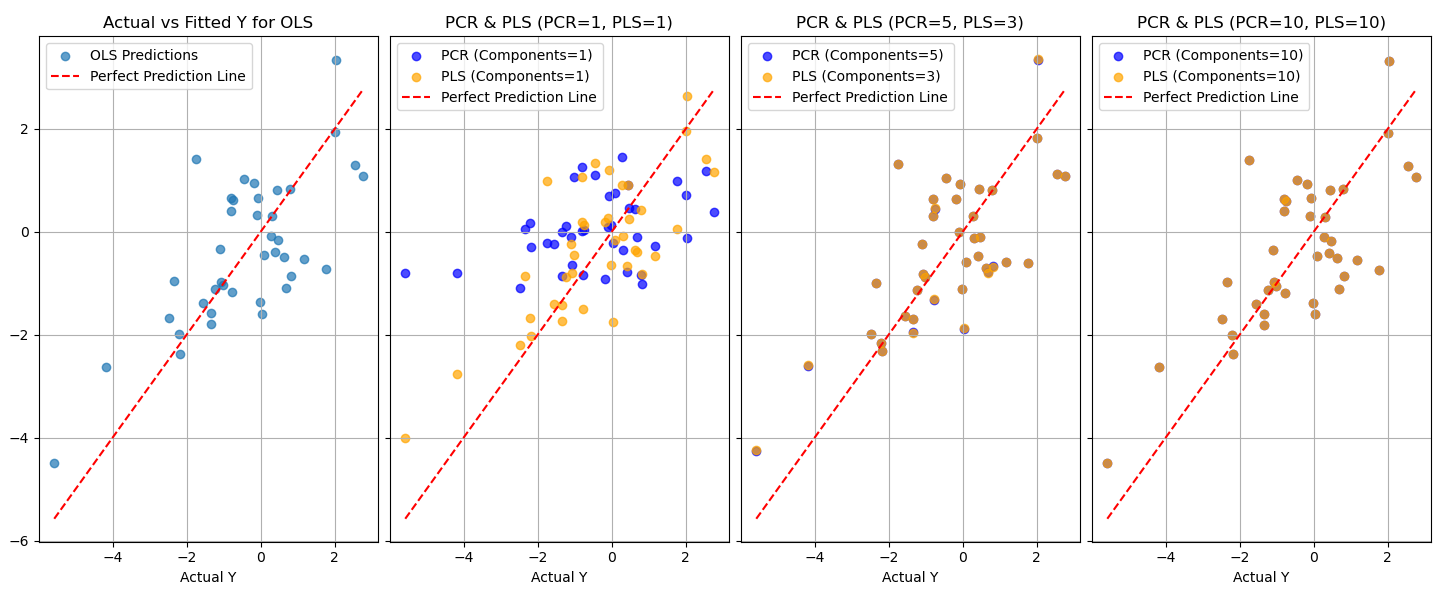
\includegraphics[width=0.9\textwidth]{Third_plot_second_simulation.png}
    \caption{Model fit: OLS, PCR and PLS}
    \label{fig:PLS_analysis}
\end{figure}


This dataset highlights the limitations of OLS in correlated predictor settings and demonstrates the advantages of PCR and PLS as alternatives. The next step is to explore how these methods perform under severe multicollinearity, where predictor correlations are extreme, and the number of observations is limited.



\section{Empirical Data Description}

For the empirical analysis, we utilize a dataset that exhibits high-dimensional characteristics, commonly found in fields such as chemometrics and finance. Specifically, we analyze a dataset containing spectral data, where the number of predictors (\(p\)) is significantly larger than the number of observations (\(n\)).

The dataset consists of:
\begin{itemize}
    \item \textbf{Response Variable (Y)}: A continuous outcome variable, representing a target measurement (e.g., concentration of a chemical compound or financial index value).
    \item \textbf{Predictors (X)}: A set of highly correlated explanatory variables, typically derived from spectral wavelengths or macroeconomic indicators.
    \item \textbf{Sample Size (n)}: 100 observations.
    \item \textbf{Number of Predictors (p)}: 200 variables.
\end{itemize}

\subsection{Preprocessing}
Before applying regression models, we preprocess the data by:
\begin{itemize}
    \item Standardizing all predictors to have zero mean and unit variance.
    \item Splitting the dataset into \textbf{training} (80\%) and \textbf{testing} (20\%) subsets.
    \item Applying cross-validation for model selection.
\end{itemize}



\printbibliography


\end{document}